\chapter{GROUPING RNA 3D STRUCTURES FROM FROM PDB USING MMCIF FILES IN RNA INTO
EQUIVALENCE SETS}

\section{Introduction}

This chapter reports changes implemented to improve modules of the data pipeline
that calculates Equivalence Classes of RNA entities of RNA 3D structures for the
Nucleic Acids Database (NDB) and for RNA.BGSU.EDU. The 3D structures are
provided by the Protein DataBank (PDB).

The PDB is an archival resource that serves as  the accumulated scientific
investigation of the 3D structures of macromolecular entities of biological
significance. The earliest entries date back to the late 1960s and early 1970s
and new entries are accumulating at an ever-increasing rate. The earliest RNA
entries were structures of dinucleotides and the latest entries include entire
ribosome structures bound to a variety of tRNA and mRNA substrates and
translation factors. But structures containing smaller RNA molecules bound to
enzymes that modify them or use them as guide RNAs  to recognize other
substrates continue to accumulate. Thus there is a huge variation in the size of
the RNA entities and of the scientific purposes for which the investigation was
conducted.

\section{Previous work}

We have previously implemented a method to group RNA molecules into equivalence
sets. The method is described in Nonredundant 3D Structure Datasets for RNA
Knowledge Extraction and Benchmarking \cite{Leontis2012b}. The current work is
an extension of these methods so, we begin by briefly describing the previous
methodology which was developed when 3D structures were still distributed in PDB
files, so that like large structures like 70S ribosomes had to be split over two
or more files. At that time it was convenient to simply select the largest chain
in a file and use to represent the RNA in the file for grouping. In cases where
the file also had one or more smaller chains the smaller ones were ignored and
no groups built for them. For example, structures of a large ribosomal subunit
contain both the 23S and 5S in the same file, the 5S was simply ignored and not
extracted and clustered separately. Each chain was compared on the basis of
sequence alignment, species and geometric discrepancy to all other chains. The
previous method did not compute all possible sequence alignments or
discrepancies due to runtime issues. The alignments and discrepancies were not
stored for future studies.

\section{Motivation for current work}

Motivation for current work
We have one main motivation for updating our RNA chain grouping method. The
first is to take advantage of technical changes data and secondly are to enhance
the scientific utility of our resources by providing a more complete set of data
that includes all chains found in RNA structures.

Recently,  PDB has migrated from “PDB” formatted structure files to the new
macromolecular Chemical Information File format (mmCIF), which made it possible
to store structural information for macromolecular complexes of any size in just
one computer file. By contrast, the out-dated PDB format was limited to no more
than 99,999 numbered atom data records per file. This change has made possible
the storage of all ribosomal subunits, large subunit, small subunit, tRNA, mRNA
fragments, 5S and 5.8S (for eukaryotes) into a single file. In some files such
as 4V4Q \cite{Schuwirth2005} more than one entire ribosome is present. Because
our old method only considered the largest chain in each file we would ignore
all chains except a single LSU. This would lead to ignoring many important
groups.

There are a number of scientific use cases for which our RNA structure classes
and derived data will be  3D structures in the PDB/NDB and these are worth
enumerating and discussing.

\begin{enumerate}
  \item Determining the breadth and depth of solved structures, ie the number of
    distinct types of RNA and the number of each type.

  \item Statistical studies of recurrent elements of RNA structure, RNA-RNA and
    RNA-protein interactions

  \item Comparative studies of similar or homologous RNA structures and
    RNA-protein complexes

  \item Functional studies of RNA structural flexibility, variation and
    conformational change in response to environmental perturbations

  \item Comparative assessment of RNA structure modeling quality and reliability

  \item Compilation of modular RNA parts for synthetic biology and RNA
    nanotechnology

  \item Analysis of  of RNA sequence variation to improve RNA structure
    prediction and understanding of RNA evolution
\end{enumerate}

Thus, the change to mmCIF format required a complete rethinking of the
procedures for extracting, naming, and clustering RNA entities and has enabled
significant improvements in the results. This chapter describes those changes
and the choices made to maximize the value of the data for diverse scientific
users.

\section{Types of molecules and requirements}

In this section we will highlight specific groups that pose special challenges
for clustering to motivate the following sections were the methods developed are
explained and their success in correctly clustering these special cases is
assessed.

\subsection{Ribosomal RNA subunits}

The largest entities are ribosomal RNAs (rRNA), which comprises the large (LSU)
and small (SSU) ribosomal subunits, the 5S rRNA, and the 5.8S rRNA in
eukaryotes. LSU and SSU from a number of species representing all three major
phylogenetic domains and mitochondria are presently available.

The rRNAs should be divided into separate Equivalence Classes (EC) as follows:
First, each of the SSU rRNAs (mitochondrial 12S, bacterial 16S and eukaryal 18S
rRNAs) should be placed into their own EC by organism. Each of the 23S rRNAs
from archaeal or eubacterial ribosomes should be placed in distinct EC. The 5S
rRNAs, which are found in the LSU of all ribosomes except some mitochondrial
ones, should also be in a separate group. While bacterial 5S rRNA does interact
directly with 23S rRNA in the LSU, it does so through non-Watson-Crick pairing
and backbone interactions involving its loop E internal loop (IL) motif and a
similar structured IL of helix 38 of 23S rRNA. The loop E of 5S rRNA has been
shown to assume the same 3D conformation in the absence of 23S rRNA and so is
not dependent on 23S to form its native state. The same holds for eukaryal 5S
rRNAs, each of which are placed in their own EC.

By contrast 5.8S rRNA of eukaryal LSU, constitutes an integral part of the large
ribosomal RNAs (26S or 28S, depending on the species), as they are homologous to
the 5’-ends of bacterial 23S rRNAs. As such they form extensive Watson-Crick
interactions with the larger rRNA of the LSU in which they occur and so,
according to the criteria defined above, belong together in the same RNA entity
, for the purposes of grouping.

In addition, the ribosome has long been an molecule of study. Early structures
\cite{Mueller2000} often were resolved at very low resolution. These structures,
while informative, are not as useful for current work as more recent high
resolution structures. While we want to group all structures it is very useful
to create groups of structures with similar resolution. In the past we have
found using resolution cutoffs of 1.5{\AA}, 2.0{\AA}, 2.5{\AA}, 3.0{\AA}, 3.5{\AA}, 4.0{\AA}, 20.0{\AA}, and
‘all’ a group of all structures regardless of resolution create useful groups.
Here we continue this practice.

From these examples we can see that the members of groups should be one or more
chains which interact extensively through watson crick base pairing should be
placed as a single entity and then grouped with other such entities. We can see
that the groups should only contain molecules from the same species. In the case
of large molecules this can be determined through sequence alignments alone.
In addition, all members of a group should fall within a resolution cutoff.

\subsection{tRNA and mRNA complexes}

tRNA molecules are commonly solved in the context of their binding to a
ribosome. In these cases they are often also bound to an mRNA fragment. These
mRNA fragments can span the A and P sites of the rRNA and have two tRNA’s bound.
The mRNA fragments (6 bases) are very small and are extensively bound to the
tRNA as all bases are paired with the tRNA. Despite this we do not want to place
the tRNA’s and mRNA into a single entity for grouping. In this case we believe
the most scientifically meaningful unit is the tRNA. The small mRNA fragment is
not interesting alone. It is small and contains no internal structure. Thus
while we do want to place two chains which extensively pair into a single unit
we do not want small unstructured chains connecting two larger structured
chains. For the purposes of grouping all chains we will allow the small
unstructured chain to ‘accompany’ the larger chains. But it should not be used
to connect the two structured chains.

The tRNA case also provides another case to consider. It is well known that some
initiator tRNA's from different species have the same sequence. This implies we
cannot use sequence alignments alone to separate molecules from different
organisms. However, there authors provide a source organism annotation.
Investigations into this annotation have showed that while many are precise some
annotations include the terms ‘synthetic compound’ or are not provided. These
chains often have identical sequence to another annotate chain. In other cases
the synthetic chain aligns very well to a correctly annotated chain. Thus we can
treat synthetic or no annotation as being similar to any other annotated
species.

These issues, the fact that some molecules from different organisms will have
identical sequences, and the potential issues with author annotations shows us
that while we should use alignments and organism assignments to connect members
of a group we must provide another criteria. We must enforce that each group
contain a single species, ignoring the assignments to synthetic. This will
maintain our requirement that groups contain only members from the same species.

\subsection{Small model compounds}

A great deal of detailed structural information has been provided by studies of
small model compounds. These compounds are often two strands which bind to form
a small helix with loops. For example studies of the isolated sarcin-ricin motif
(CITE: 4NLF) have provided detailed information on its structure. In these
structures the unit we should cluster is the duplex. Like the LSU and 5.8S each
strand interact extensively through Watson-Crick base pairs. However, these
strands have no internal structure. There are also model compounds, such as the
nano square that are composed of 8 chains \cite{Dibrov2011a}.

From these examples we can see that we should be able to join any number of
unstructured chains together to form a single unit for grouping. This is
different from the case of multiple tRNA's on a small mRNA fragment where the
two tRNA's would not form a single unit. Here we want the chains, even if they
are not directly interacting, to form a single unit.

Many of these small model compounds differ from one another from due to single
nucleotide changes. These changes are intentional and so we require that small
molecules have identical sequences in our grouping.

\subsection{Small Protein and RNA complexes}

Several proteins have been solved with small bound RNA's. These RNAs are often
poly-A or other such simple sequences. These chains may agree in sequence and
species assignments but they differ in assigned geometry due to binding by the
protein. These chains should be split even if they are similar on the basis of
sequence and species. Thus our groupings should be sensitive to the overall
geometry of the members.

\section{Criteria for equivalence classes and their members}

These examples show first of all, that many CIF miles contain more than one
chain. Second the example of Eukaryotic LSU rRNA show that the members of some
EC may be one or more chains in contrast to our previous EC. A prerequisite of
grouping is to define the RNA-containing entities to be extracted from structure
files as precisely as possible and in a manner that is biologically relevant for
the purposes of most users of the resource. Guided by giving priority to
biological relevance, we settled on the following definition of the relevant
RNA-containing entities: The entities to be identified and extracted from
PDB/NDB structure files are “groups of one or more RNA chains that form
identifiable integrated structural and functional units.” Internally we refer to
these entities as “RNA integrated functional elements” or “RNA IFEs.” We will
use the term “IFE” as a short-hand for this definition.  Most RNA IFEs consist
of a single chain, but some do not. The simplest examples comprise two chain
Watson-Crick paired chains forming a duplex structure: strictly, this comprises
two molecules, but effectively it is a single entity or RNA IFE.

From these examples we can see there are 3 requirements for each EC.
\begin{enumerate}
  \item Two IFE’s included in the same Equivalence Class should come from the
    same biological source. The intention of this criterion is to separate
    homologous RNA molecules, for example SSU rRNAs from different organisms,
    into distinct Equivalence Classes.

  \item Two IFE’s included in the same IFE should have very similar, though not
    necessarily identical sequences. This criterion may seem redundant with the
    first criterion. The intention is to include sequence variants (for example
    16S rRNAs coded by different genes of the same micro-organism that differ in
    a small number of positions) but to separate molecules with similar
    sequences from evolutionarily related organisms that belong to distinct
    species. We note that not all RNA chains in PDB are labeled with a
    biological source, which complicates clustering.

  \item Two IFE’s included in the same Equivalence Class should have the similar
    conformations and geometries. The intention of this criterion is to separate
    instances in which there is a significant conformational change, even when
    the RNA sequence(s)and biological source  are the same. For example, poly-A
    bound to poly-A binding protein (PAB) (PDB 1CVJ) has a different
    conformation from poly A forming a parallel strand duplex (PDB 4JRD). These
    IFE’s are structurally dissimilar and should not be in the same equivalence
    set, even though the sequence may be identical.

  \item Two IFE’s included in the same EC should have similar resolution.
\end{enumerate}

However, we decided to group structures together even though their sizes differ
when:

\begin{enumerate}
  \item The same molecule was used in the experiment as reported in the CIF data
    field ``poly\_seq\_scheme''. In some cases only part of the molecule was
    resolved. Because the experiment was using the same molecule we believe it
    should be grouped with the other structures of the same, but larger
    molecule.

  \item The observed part superposes well with the corresponding parts of more
    completely resolved structures.

  \item The observed structure is a small part of the overall molecule. For
    example, there are structures of a single domain of the ribosome
    \cite{Nissen2000}. These structures are best grouped with the other
    ribosomal structures as that is the context they are just a small portion of
    the larger complex.
\end{enumerate}

In addition, there are several other cases where we assign IFE’s to the same
equivalence set:

\begin{enumerate}
  \item We group IFE’s together EVEN WHEN their geometries differ significantly
    when the structures are too low resolution as the data are not adequate to
    quantify the structural differences.

  \item Structures belong together even when RNA is bound to different proteins
    or ligands but they have when they have very similar geometries. At present,
    it is not our intention to classify PDB structures at the level of
    RNA-protein complexes. For this study we focus on the RNA components of the
    structure.
\end{enumerate}

There are several important implications of these requirements. First it is
possible that the homologous RNA molecules (for example iso-accepting tRNAs)
from different species have nearly identical sequences and structures.
Nonetheless they will be placed in different groups In addition, it is possible
that two groups will have similar sequence and species but differ only in
geometry.

\section{Methodology for building Equivalence Sets}

In this section we discuss the process of building equivalence sets. The overall
process is to
\begin{enumerate}
  \item Identify and extract RNA chains

  \item Build RNA IFE's from individual chains.

  \item Link pairs of IFE's by sequence similarity, source species, and
    geometric similarity.

  \item Extend equivalence sets using transitivity of similarity links

  \item Assign names

  \item Display data on our Website

  \item Share data with NDB
\end{enumerate}
Below we discuss each step in detail and how it achieves our goals.

\subsection{Building RNA IFE's from individual chains}

We have implemented an algorithm for joining chains into IFE's. As discussed in
our examples the joining logic depends on whether or not a chain is
``structured''. Structured chains only get joined with other structured chains
they directly interact with, and they must make a significant number of
interactions with them. Unstructured chains are always joined any chain they
interact with, but they will not indirectly join two structured chains together.

Our algorithm operates as follows. We first mark all chains in a structure as
``structured'' or ``unstructured''. A ``structured' chain is defined by having at
least 5 internal (within the same chain) cis Watson Crick/Watson Crick (cWW)
basepairs. We then join chains based upon a few rules. A representation of these
rules is shown in Figure~\ref{fig:build-ife}.

\begin{figure}
  \includegraphics[width=\linewidth]{chapter-3/figs/build-ifes}
  \caption{The rules for building connecting chains into IFE's. Each chain is
    represented by a circle. Unstructured chains are in blue with the letter
    ``U'', while structured chains are orange in ``S''. The left side indicates the
    input and the right shows the possible results of each case. On the left the
    dotted lines indicate one or more cWW interactions between the chains. On
    the right each grey circle indicate an IFE built of the two chains. For case
    1 and 2 we always join the two chains into one IFE, while in case 3 it
    depends upon the number of interactions. Case 4 shows that for two
    structured chains selected by an unstructured chain the two structured
    chains are placed in separate IFE’s while the unstructured chain is placed
  in both IFE's.}
  \label{fig:build-ife}
\end{figure}

In this figure we can see the four basic cases. First when determining if we
unstructured chains should be connected, we always connect them if they have any
cWW interactions between them. This allows for joining of separate stands of
duplexes. In the second case we always connect unstructured chains to structured
chains. This serves to connect unstructured fragments such as mRNA’s to the
structure tRNA’s they are interacting with. For connecting two structured chains
we require that the maximal ratio of external cWW to internal basepairs is at
least 0.6. This is an experimental determined cutoff. It may be adjusted in the
future. To examine if this cutoff is reasonable we produced the figures shown in
Figure~\ref{fig:ext-vs-int}.

\begin{figure}
  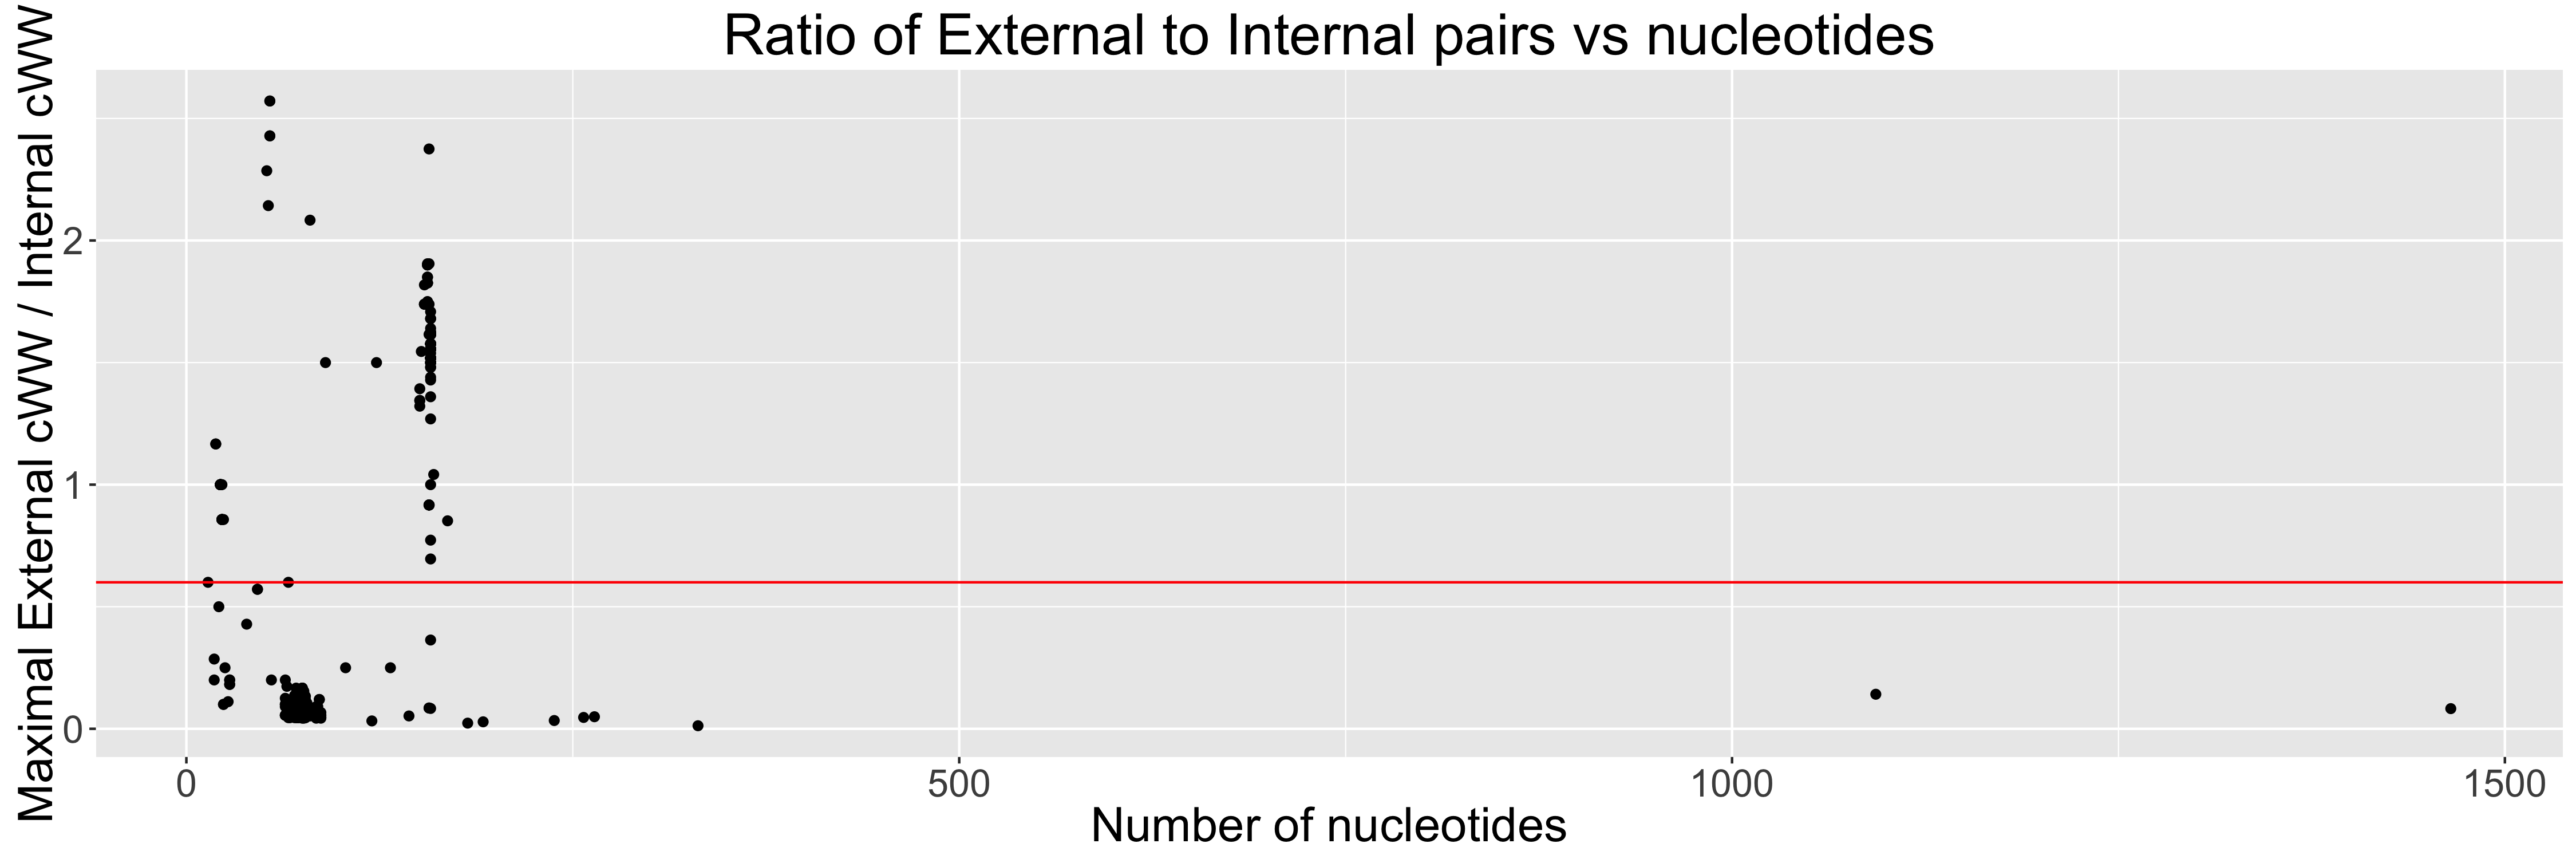
\includegraphics[width=\linewidth]{chapter-3/figs/internal-external}
  \caption{Summary of the ratio of external to internal base pairs. The leftmost
    panel shows a histogram of the maximal ratio of external to internal pairs
  for all pairs of chains which have an interaction between them. }
  \label{fig:ext-vs-int}
\end{figure}

\subsection{Connecting pairs of IFE's to from equivalence sets}

To build equivalence sets we compare all pairs of IFE’s based upon their species
assignments, their alignment, their discrepancy. Pairs of chains which have a
valid alignment, are from similar species and have a discrepancy of less than
0.4{\AA}, if computed, are joined. We then build the EQ sets by placing all chains
which are transitively connected into one set.

The steps are:
\begin{enumerate}
  \item Determine the species assignment for all chains.
  \item Compute the alignment of all pairs of alignable chains.
  \item Compute the discrepancy between all chains which have a good alignment
\end{enumerate}

The first step requires looking up the assigned phylogeny for chain. Many chains
are assigned to a particular species making the lookup trivial, however some are
assigned to a subspecies. For these cases we use the parent species of the
chain. However, not all chains are assigned to an organism, many are marked as
‘synthetic construct’ or not assigned any organism. In both of these cases we
treat the organism as synthetic. In addition, a few chains (3) are assigned to a
genus rather than a species or sub-species, in these cases we treat the chain as
being synthetic as well.

In order to compute the alignments between all pairs of chains correctly and in
a reasonable time frame we align experimental sequences. Experimental sequences
are the sequences used in the experiment and may differ from what is observed in
the experiment. Often the solved structure will have ‘gaps’ indicating where
bases were not resolved. For example EXAMPLE. In order to build alignments
correctly we use the experimental sequence. If we did not we would have to
ensure that the resulting alignments respected gaps in the both chains. The
alignments would  have to have breaks where the observed chains have breaks.
This is a difficult problem and it is simpler to use the experimental sequences
where this is not a concern.

In addition, by using experimental sequences we reduce the number of required
alignments. It is very common to use the same molecule in many experiments. For
example, there are many structures of the same E. coli ribosome with different
tRNA’s or antibiotics. All of these structures can be represented by a few
experimental sequences. There is no need to realign sequences simply because
they came from different experiments, the alignments will be the same.

We also require that all the pairs of experimental sequences to align  have
similar size. The rules for size depend upon the size of the chain. The specific
rules are shown in TABLE SIZE RULES. The reason for the size constraint is to
reduce the number of required alignments while ensuring that we perform all
required alignments. For our purposes an alignment between a large and small
subunit will never provide any information so we avoid computing them.

Finally, we require that the experimental sequences have either been assigned to
the same species or one of them has been assigned to synthetic. We refer to this
as the chains having a similar species. This ensures that we are only comparing
sequences which could be from the same source. We have observed that some
experimental sequences are assigned ‘synthetic’ in one experiment are assigned a
species such as E. coli in another experiment. Thus we allow the comparison of
synthetic chains to any other chain, so long as it has similar size. The last
step is to compute the discrepancy. Discrepancy is a measure of geometric
similarity like RMSD but it is sensitive to the base orientation and position.
It has been used extensively in our lab for searching RNA 3D Structures
\cite{Sarver2008a}, building NR sets in the past \cite{Leontis2012b}, as well as
building motif groups \cite{Petrov2013}. We only use the first structured chain
in each IFE. While this is a simplification of the situation it has proven to
work well and makes the problem simpler. For discrepancy we are only interested
in chains that:

\begin{enumerate}
  \item Have a good alignment between them. As this discrepancy will be used to
    build EC, there is no need to compute it for chains that do not align well.
    These chains cannot be in the same EQ set so discrepancy is not needed. This
    reduces the number of comparisons needed making the computations much
    quicker.

  \item Have resolution less than 4.0{\AA} or are solved using NMR. We do not
    compute discrepancies for chains with poor resolution (greater than 4.0{\AA})
    because doing so provides artificially inflated value. Many structures of
    low resolution are helices which have not been modeled with planar paired
    bases. This modeling is inaccurate and produces high discrepancy when
    compared to carefully modeled helices. Because of this we split structures
    which should be joined. We however, do allow for comparisons using NMR
    because most NMR structures are very small and the errors introduced are
    small.

  \item Have at least 3 aligned bases. This is because discrepancy is only
    defined for at least 3 bases.

\end{enumerate}

With these rules we are able to efficiently compute all required discrepancies.
By doing this as part of our pipeline we are able to store these values. This
allows for comparison of grouping methodologies and constraints.

We then connect all pairs of IFE’s which satisfy the alignment, species and
discrepancy requirements. These connections are treated as a graph and used to
build equivalence classes through transitivity.

\subsection{Building equivalence classes from pairs of IFE’s}

We build EC through transitivity. This means that all connected IFE’s, even if
the connections are indirect, are placed into a single group. An example of such
a clustering is shown in Figure~\ref{fig:transitivity}.

\begin{figure}{ht}
  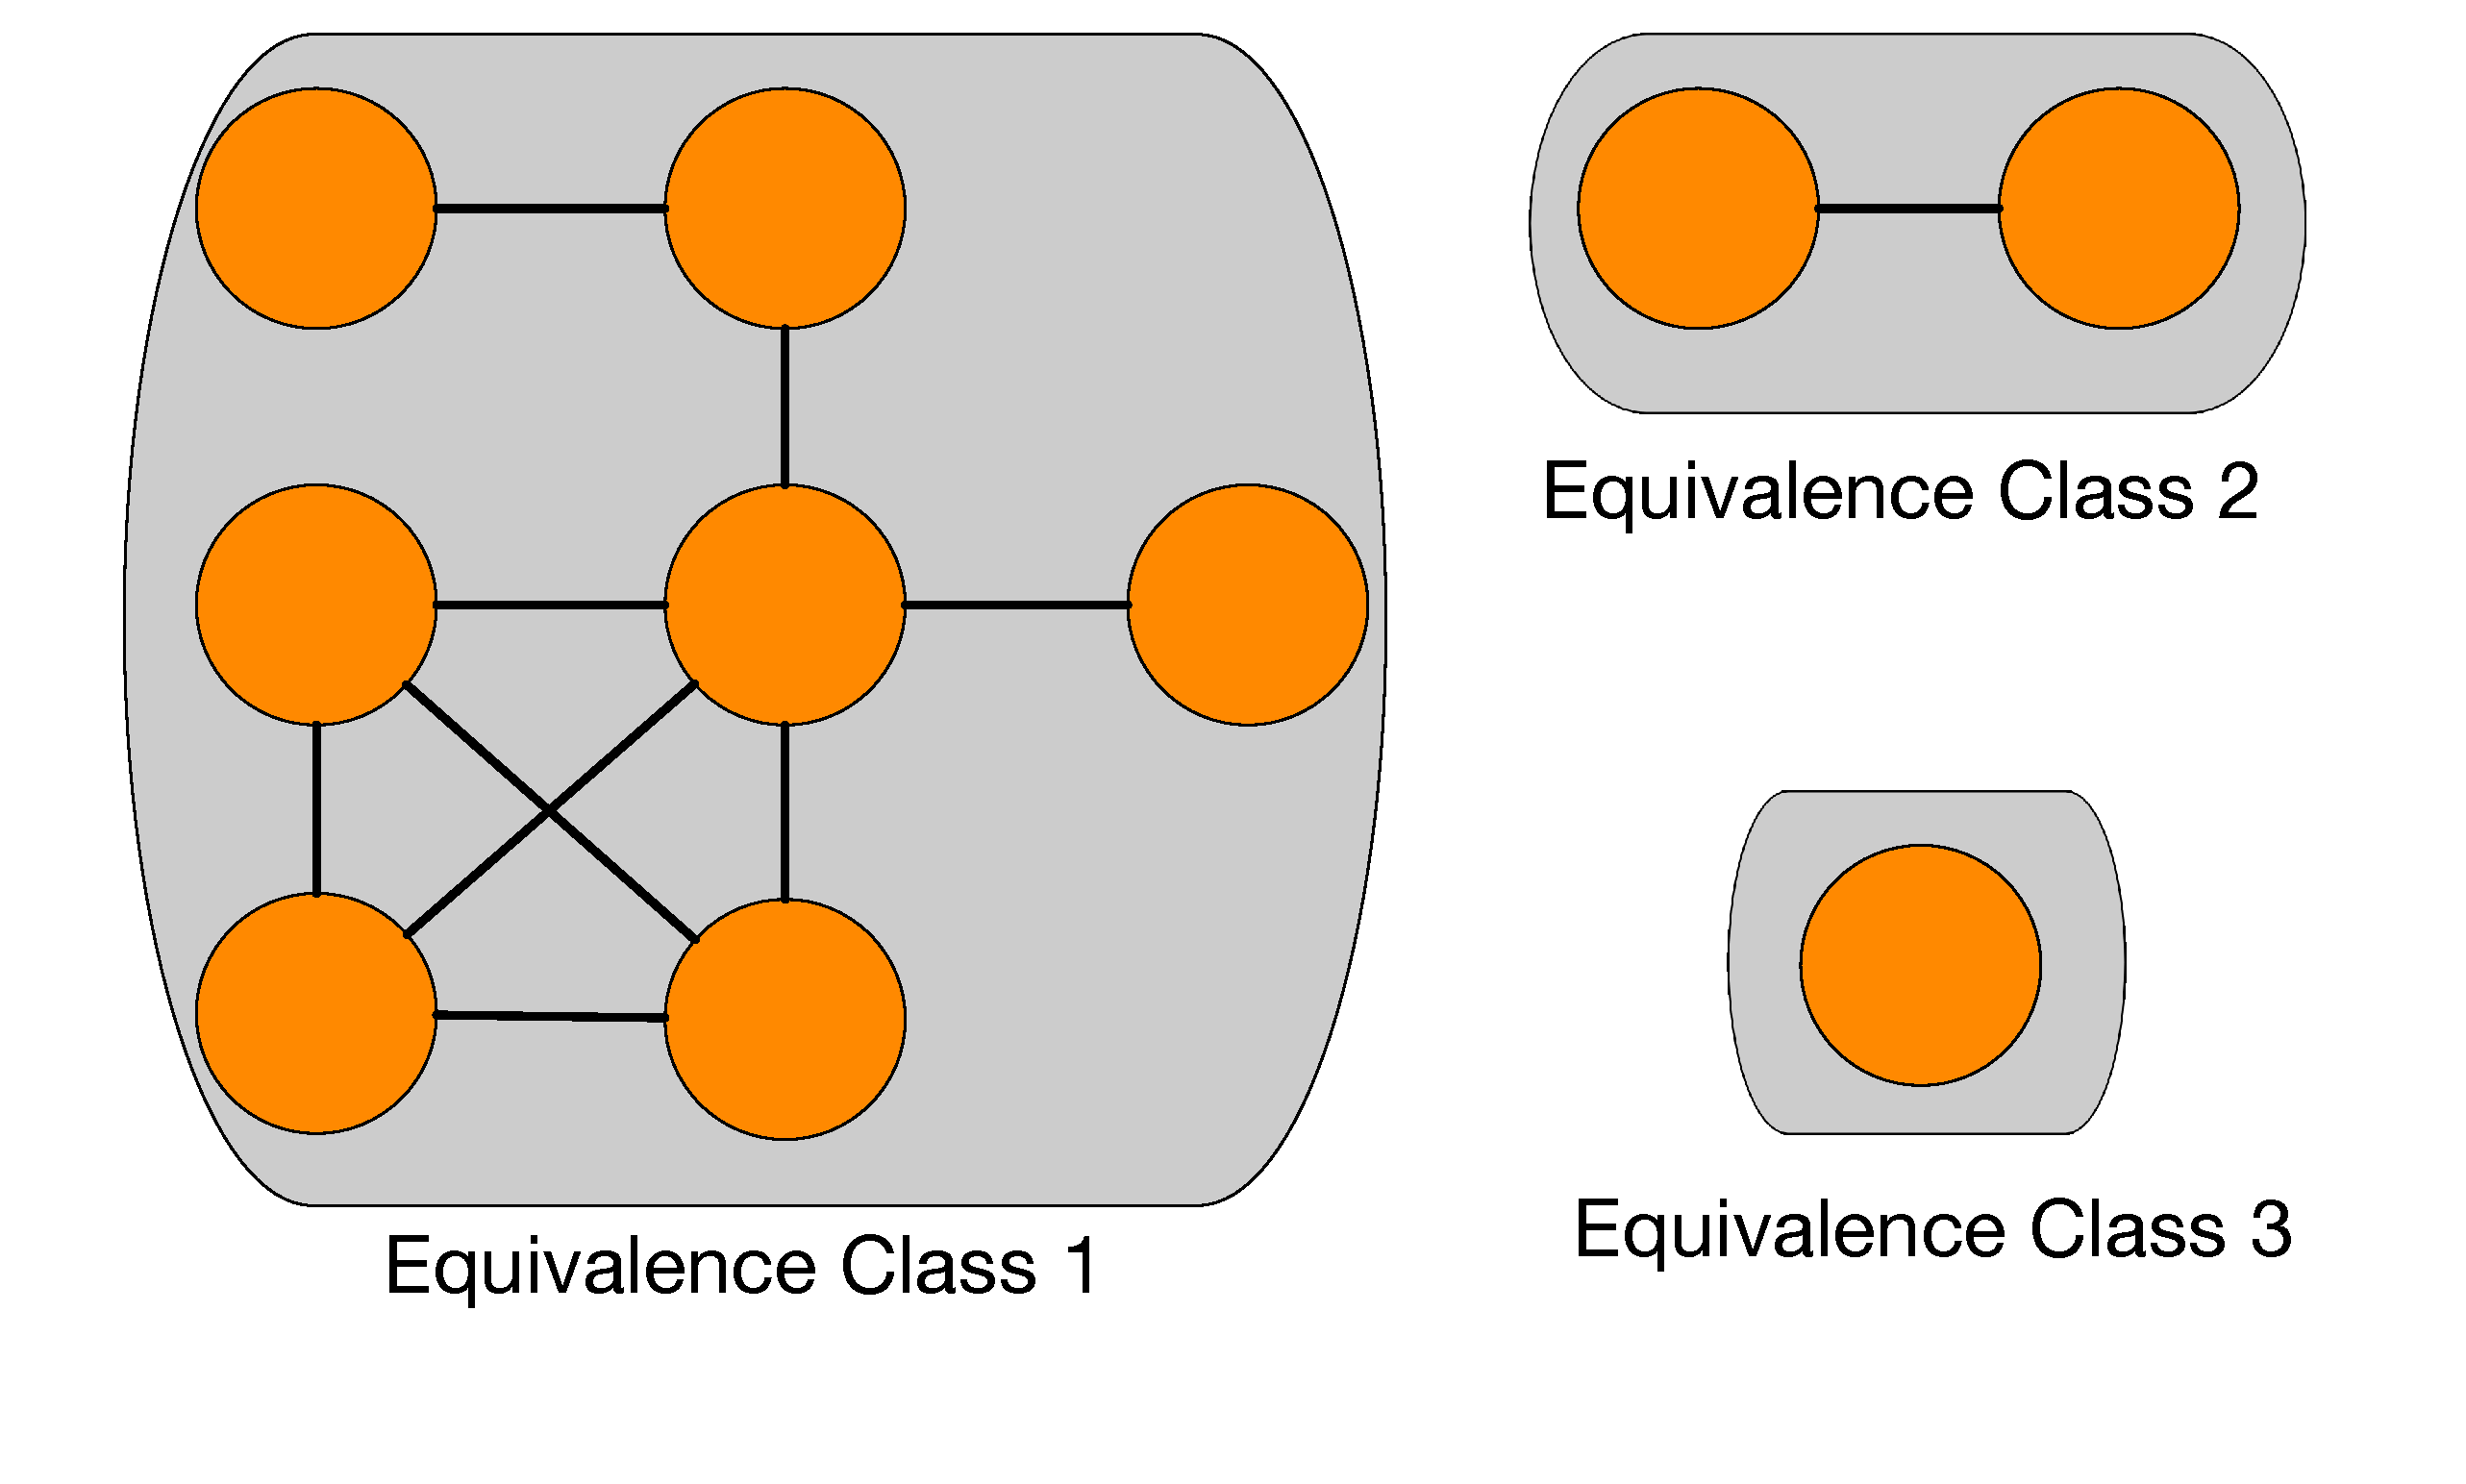
\includegraphics[width=\linewidth]{chapter-3/figs/ife-transtivity}
  \caption{Schema of Equivalence Classes built by transitivity. In this figure
    each IFE instance is represented by a circle.Lines connecting circles
    indicate pairs of IFE's having similar sequences, the same species and
    geometric discrepancy below the threshold value of 0.4. Each Equivalence
  Class is represented by the grey background around a set of circles. To in
included in a class an instance need only be connected to one other member of
the class.}
  \label{fig:transitivity}
\end{figure}

Using transitivity minimizes the number of singleton outlier groups. Most IFE’s
will compare well to at least one other, placing them in the same group. The use
case of studying structural variation in molecules. Without a transitive
grouping, structures which differ only in structure would be split from all
other instances. The groups are created using all possible structures, the ‘all’
resolution cutoff. From there the groups are filtered to only contain structures
which satisfy each resolution threshold. With the groups created, the only
remaining step is to name them

\subsection{Naming equivalence sets}

In previous work Dr. Anton Petrov created a naming scheme based upon the
parentage of the equivalence class \cite{Petrov2013}. I preserve the overall
scheme but have modified it in a significant way to make an easier to understand
system, as described next.

The naming scheme is as follows:
``NR\_{resolution\_cutoff}\_{unique\_handle}.{version}''. This scheme has 3
components, the resolution cutoff used, a unique randomly selected handle and
the version number for this group. The resolution cutoff provides information on
what the resolution is used to build the EQ set. The unique handle is a unique
randomly generated number that serves to make all ids unique.

We have changed the naming scheme so that the unique handle is identical across
all resolution cutoffs of the same set of structures. For example, an EQ set
built of tRNA’s at the ``all'' resolution cutoff may have the name:
``NR\_all\_00001.1''. At the 4.0{\AA} resolution cutoff this now would have the
name ``NR\_4.0\_00001.1''. This differs from the previous method where as
different randomly generated handle was assigned to each resolution cutoffs of
the same equivalence set. By making this change the random handle remains
identical across resolution cutoffs making it much easier to which EQ sets have
the same molecule.

\section{Results of Equivalence Set building}

For the purposes of this chapter we created an EQ grouping using all structures
available as of July 25, 2016. This grouping was then analyzed to see how the
resulting groups matched our objectives. I begin with a general description of
the clustering and then discuss each previously mentioned case in detail,
finally I examine the groupings of outliers.

\subsection{General properties}

I built a grouping using all PDB available from July 28, 2016. The grouping used
3213 PDB’s which contained 7015 IFE’s. These were grouped into 2168 EC’s. These
groups varied in size from 1 (singleton groups) to 377 instances. A summary of
the member count distribution is shown in in Table~\ref{tab:eq-size-dist}.

\begin{table}
  \begin{tabular}{lr}
    \toprule
    Number of instances & Number of Equivalence Classes (Percent of all classes) \\
    \midrule
    1               & 1352 (62.4\%) \\
    2-5             & 615 (28.3\%)  \\
    5-10            & 118 (5.4\%)   \\
    10-20           & 53 (2.4\%)    \\
    20-50           & 16 (0.7\%)    \\
    \textgreater 50 & 14 (0.6\%)    \\
    Total           & 2168 (100\%)  \\
    \bottomrule
  \end{tabular}
  \caption{Counts of the number of classes for a range of sizes. This table
    shows the number of classes for a range of sizes for the new grouping method
  for all 3213 structures available as of July 28, 2016}
  \label{tab:eq-size-dist}
\end{table}

The table shows a surprisingly high percentage, 62\%, of singleton groups. I
tested to see if this is consistent with the previous method by building a
grouping using the set of structures December 05, 2014 as shown in Table COMPARE
SIZE DIST. This date was chosen because it corresponds to both the last grouping
using our previous method as well as as the transition to mmCIF data. These two
datasets contain the same experimental results, however there are fewer mmCIF
files because many  of the PDB files have been merged into a single mmCIF file.
This gives us an ideal set to compare the two methods. From the table we can see
that the old and new method have similar performance, with the new one having
fewer singleton groups. Thus 62\% of our groups are singleton groups for the July
28, 2016 data is not surprising when compared to the previous groupings.

\begin{table}
  \begin{tabulary}{\linewidth}{LRR}
    \toprule
    Number of instances & 
    Number of Equivalence Classes in 2.0 & 
    Number of Equivalence Classes in 1.89 \\
    \midrule
    1               & 1081 (61.0\%)  & 1112 (78\%) \\
    2-5             & 527 (30.0\%)   & 234 (16\%)\\
    5-10            & 88 (5.0\%)     & 31 (2\%)  \\
    10-20           & 38 (2.0\%)     & 19 (1\%)  \\
    20-50           & 20 (1.0\%)     & 8 (0.5\%) \\
    \textgreater 50 & 11 (0.6\%)     & 5 (0.3\%) \\
    Total           & 1765 (100\%)   & 1409 (100\%) \\
    \bottomrule
  \end{tabulary}
  \caption{Comparison of new method to previous method. This table compares the
  performance of the previous and new method on the same data set of structures.
The data are taken from
\url{http://rna.bgsu.edu/rna3dhub/nrlist/download/2.0/all/csv}, which contains 2680
structures, and \url{http://rna.bgsu.edu/rna3dhub/nrlist/download/1.89/all/csv}
(contains 3145 structures) and represents all the structures available as of
December 5, 2014. The transition from 1.89 to 2.0 corresponds to the move from
PDB to mmCIF formats which decreased the total number of files, because many
previously separate files were merged}
  \label{tab:eq-size-dist}
\end{table}

I next moved to examine results of groups of particular interest. I begin with
the ribosomes, then tRNA’s, and then protein/RNA complexes.

\subsection{Ribosomal subunits}

As an example to evaluate the groupings of ribosomes, I examined the equivalence
classes containing the Thermus thermophilus small ribosomal subunit (SSU). We
constructed heatmaps of both the sequence similarity and the discrepancy between
all chains as shown in Figure~\ref{fig:tt-ssu-align} and
Figure~\ref{fig:tt-ssu-disc}. The alignment heatmap indicates the high sequence
similarity among all IFE’s. The geometric discrepancy heatmap shows that there
may be two main structurally groups in the equivalence class. Currently we are
exploring these groups to see if they correlate to biological states.

\begin{figure}[h]
  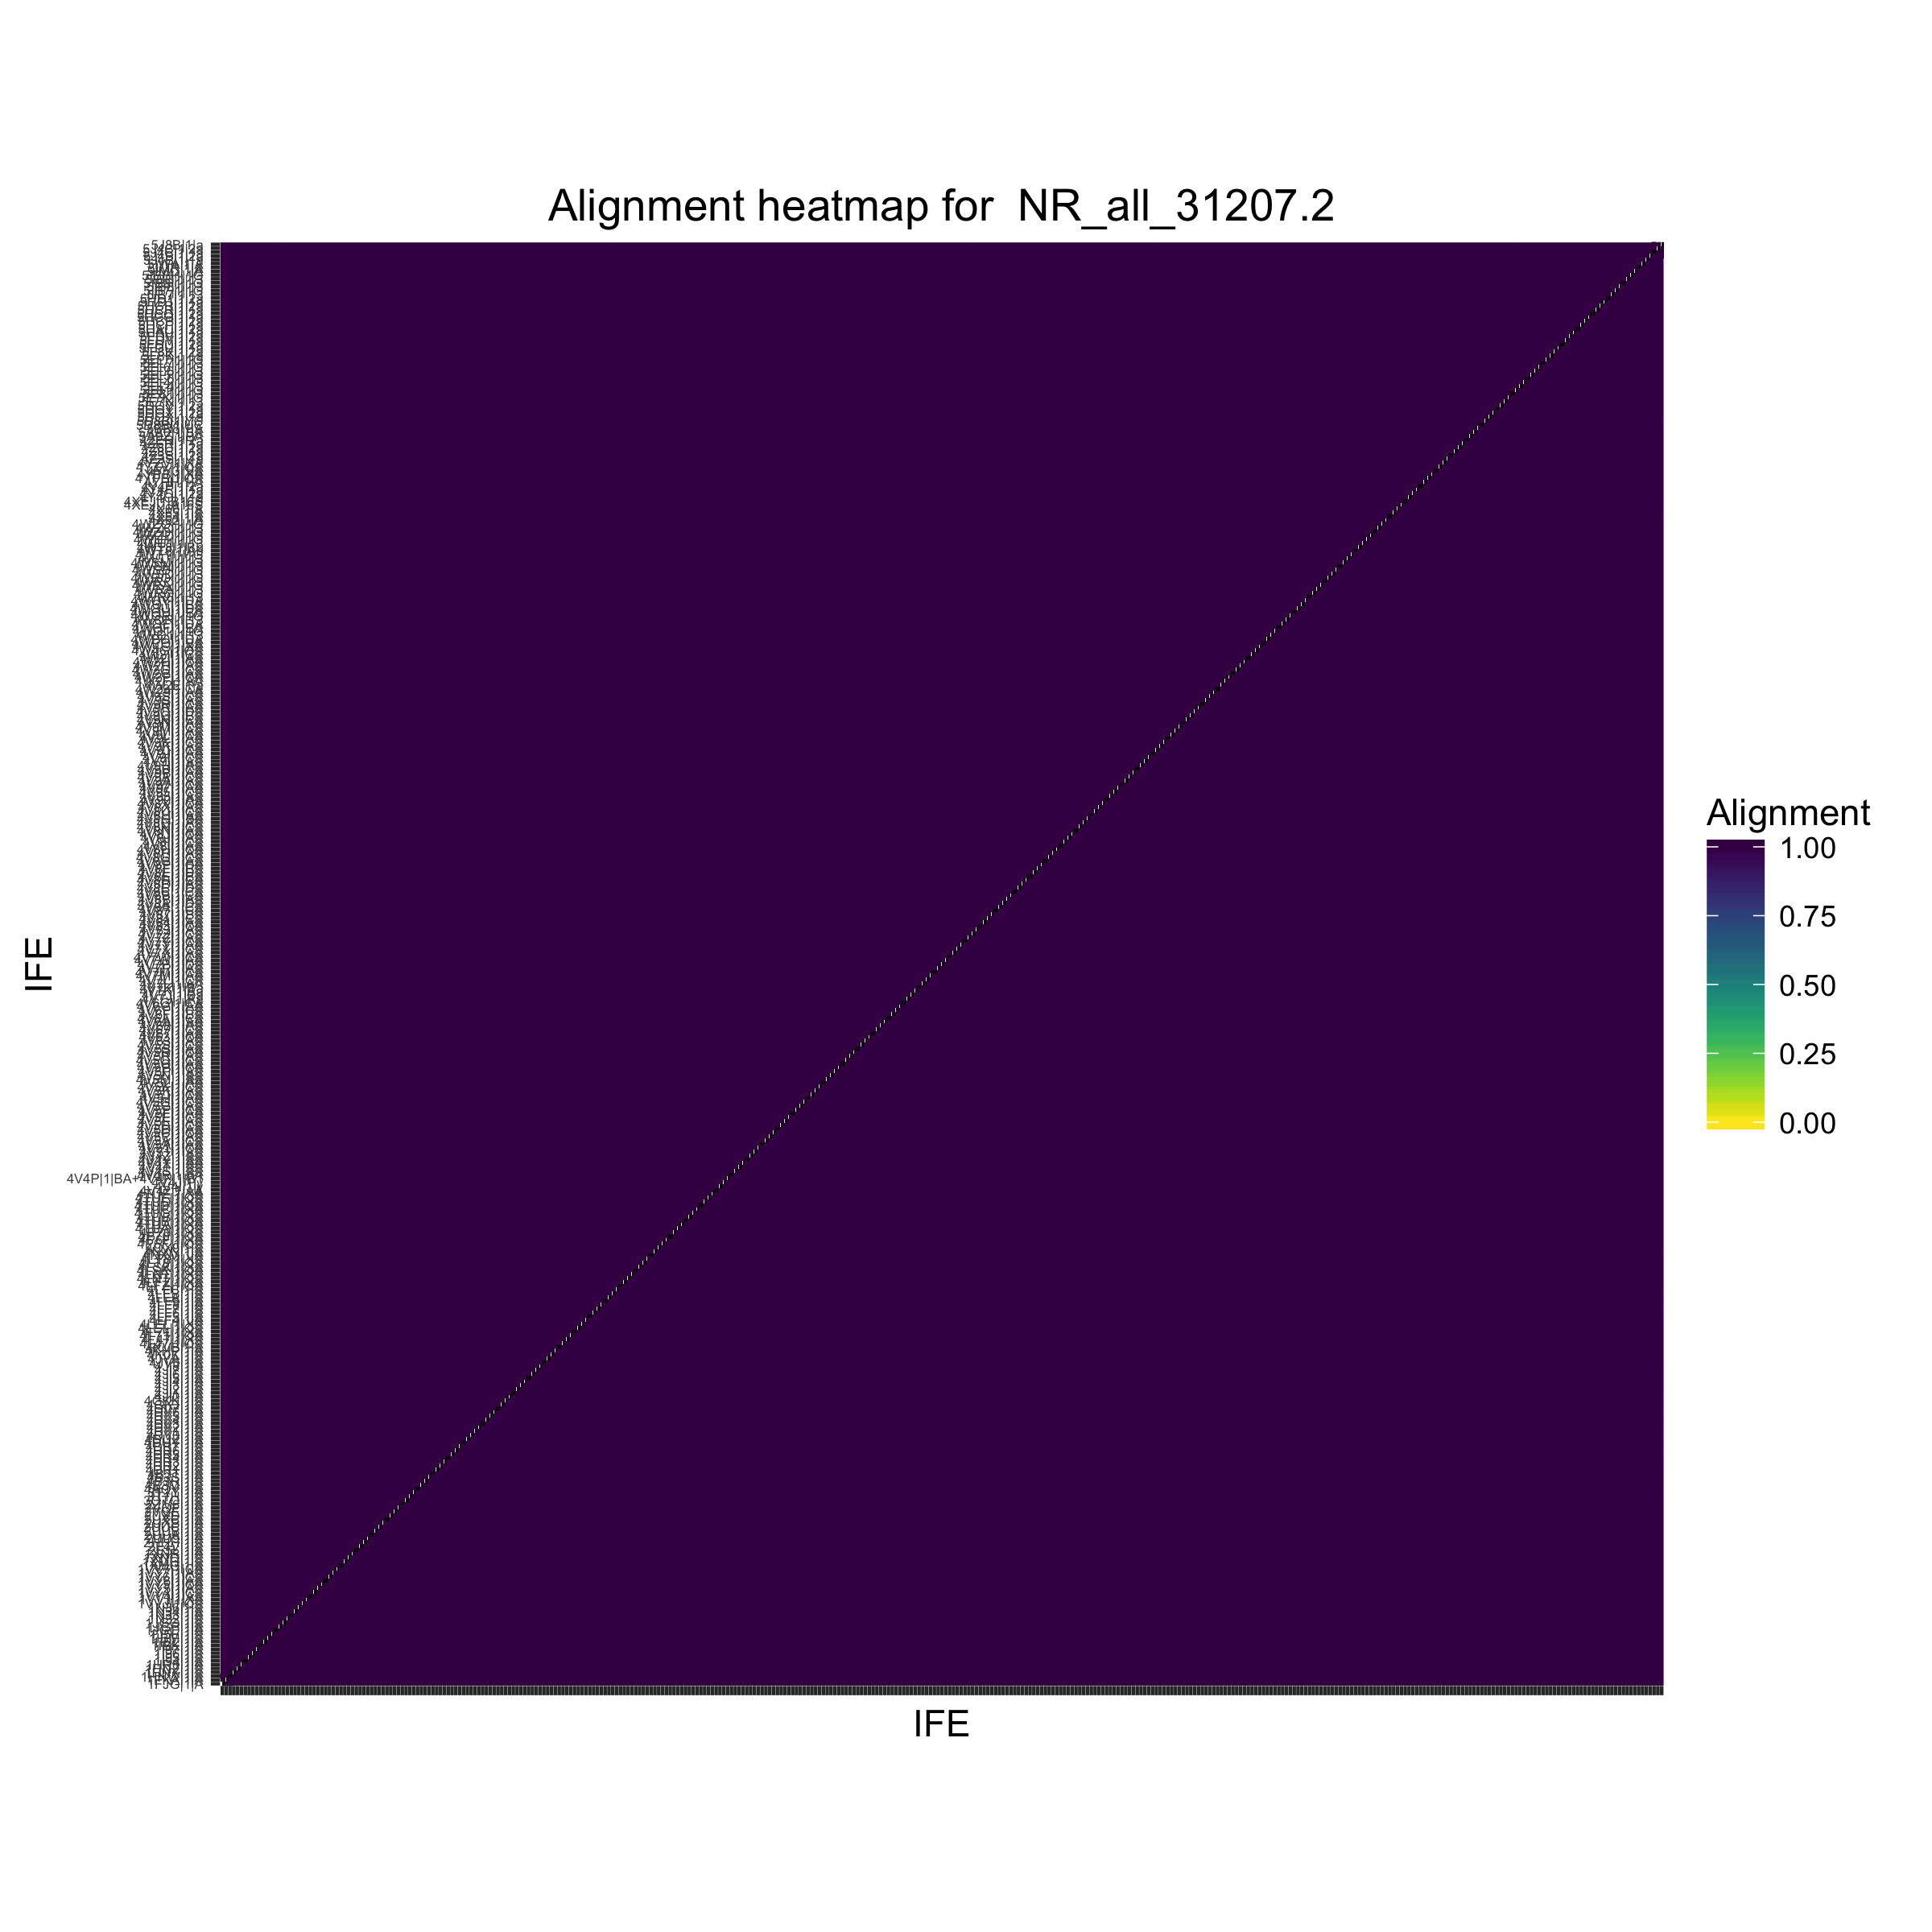
\includegraphics[width=\textwidth]{chapter-3/figs/tt-ssu-align}
  \caption{A figure summarizing the sequences similarity for all IFE’s in the
    Thermus thermophilus small subunit. Color scale indicates discrepancy
  values, lighter colors being worse.}
  \label{fig:tt-ssu-align}
\end{figure}

\begin{figure}[h]
  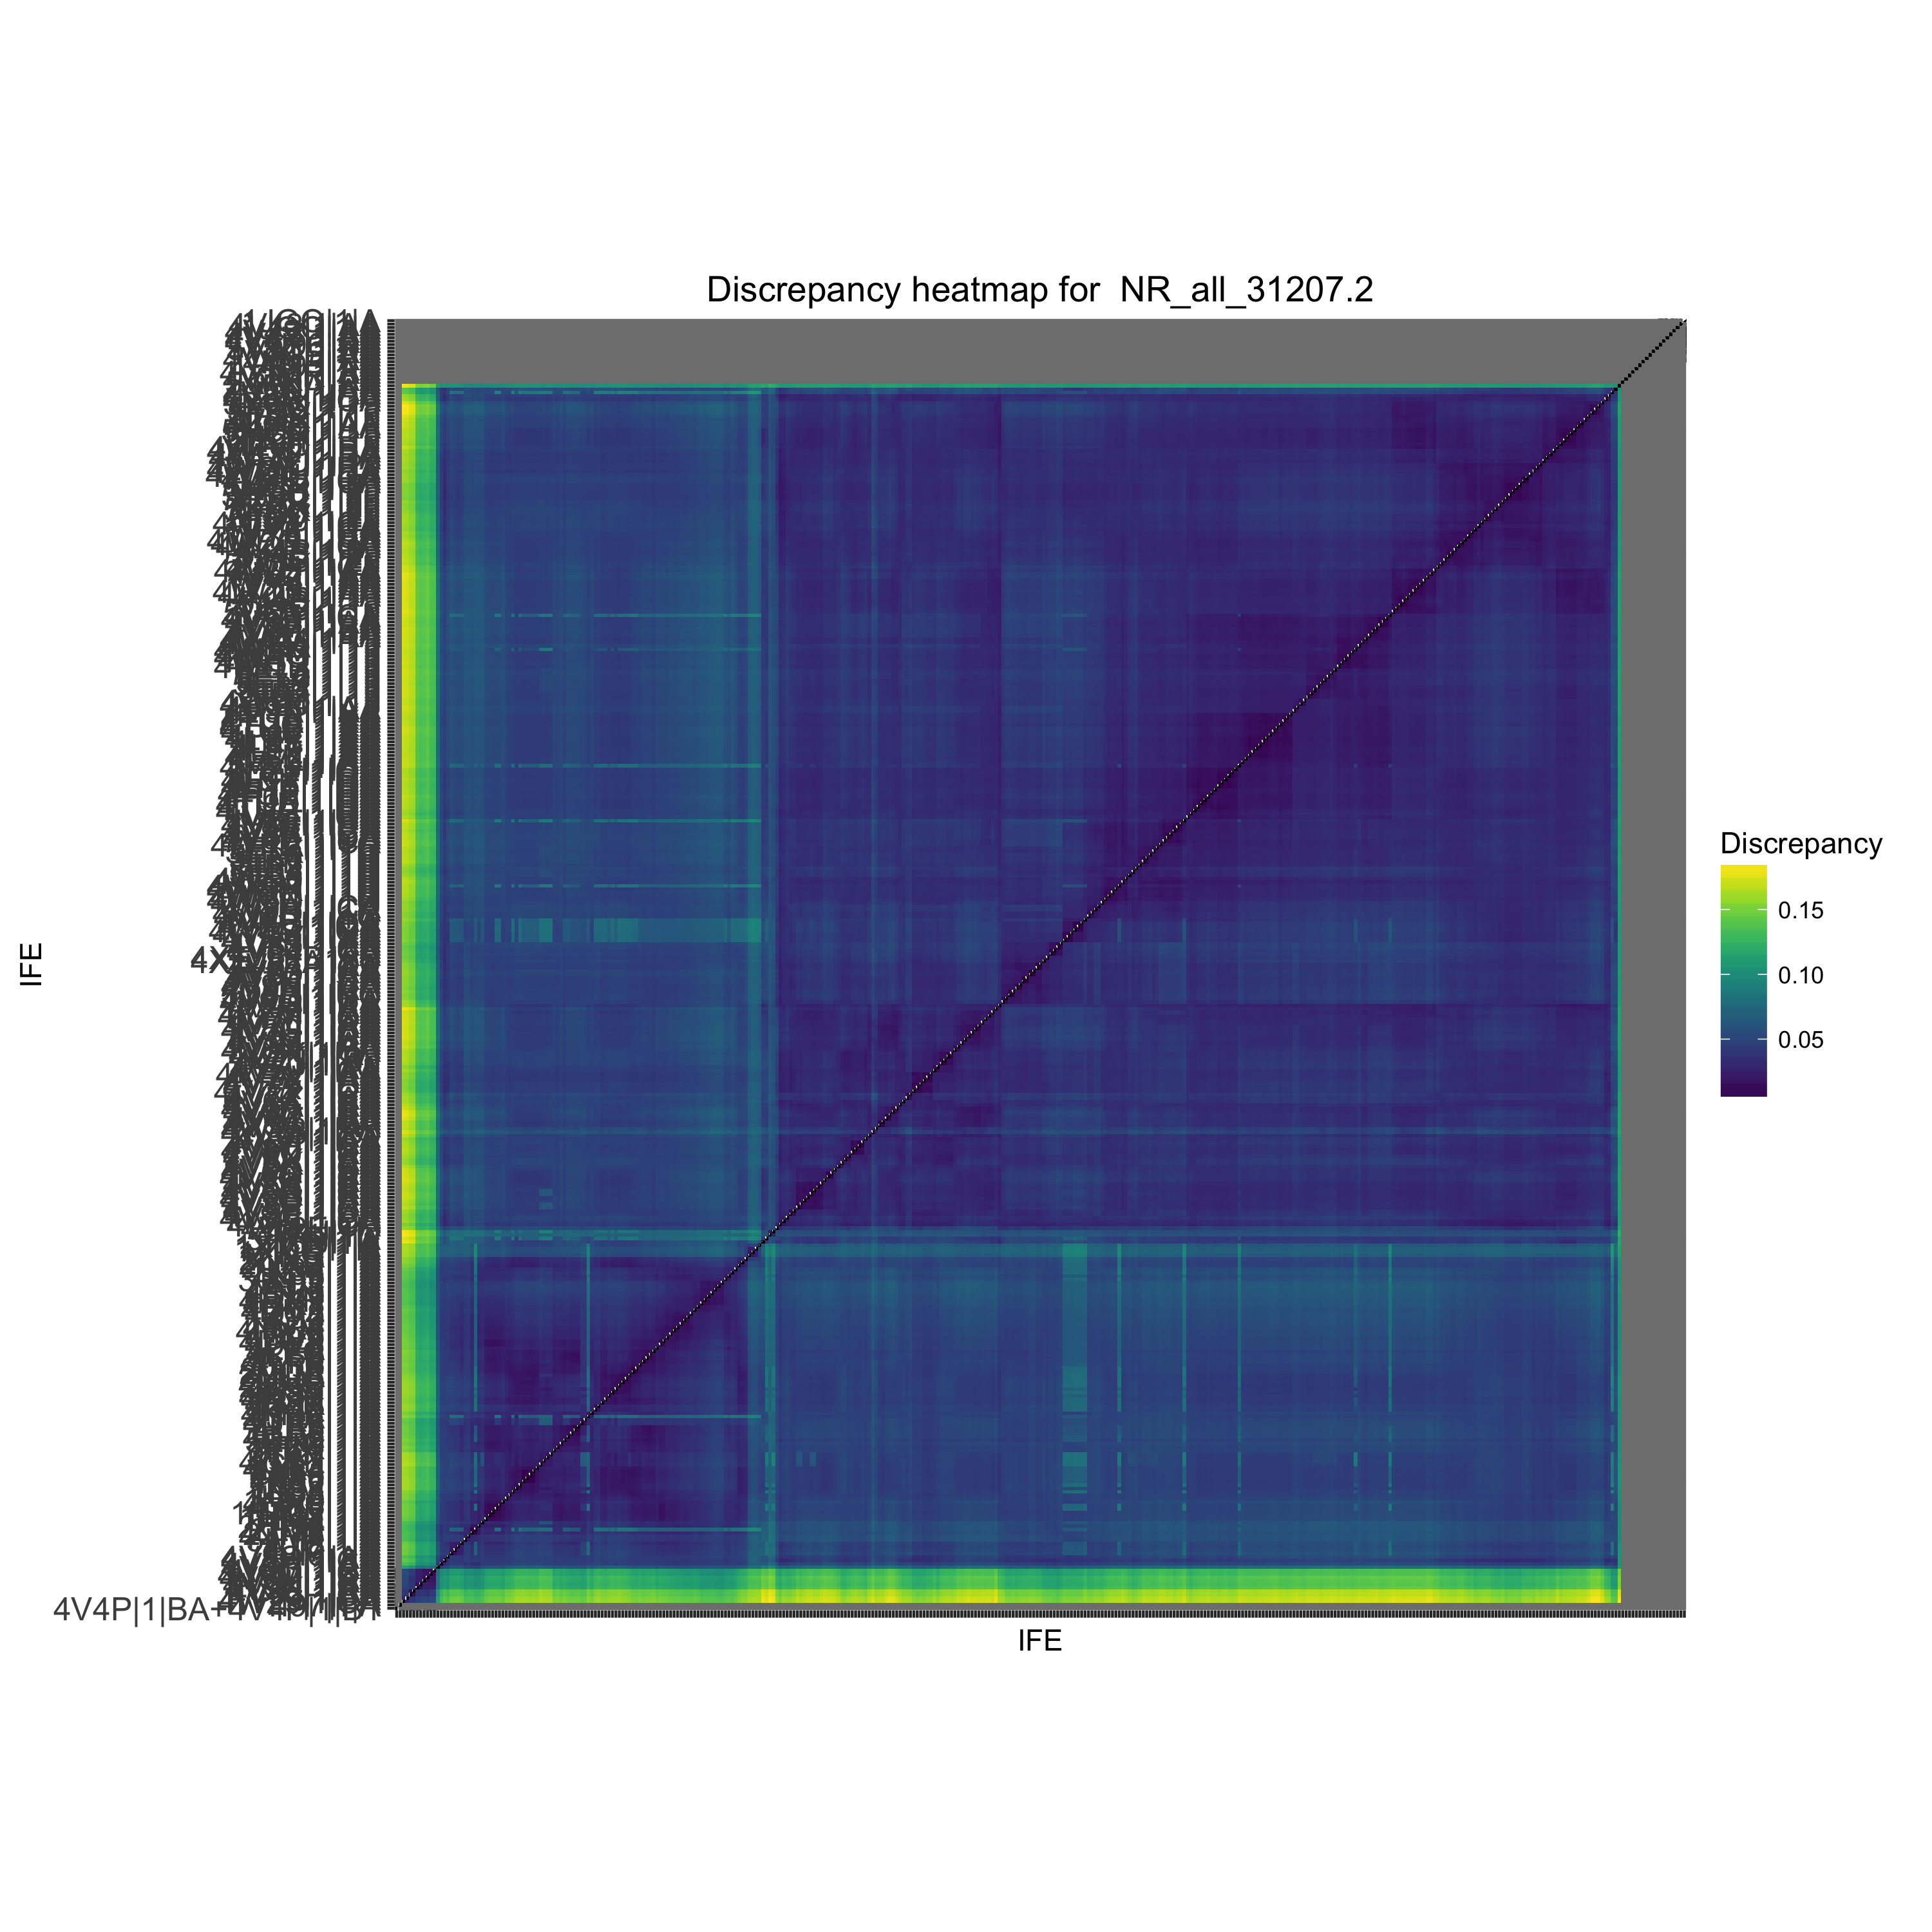
\includegraphics[width=\textwidth]{chapter-3/figs/tt-ssu-disc}
  \caption{Summary of the discrepancy for all pairs of IFE’s in the Thermus
    thermophilus small subunit. Grey squares indicate no data computed, because
    that structure has too low a resolution. Color scale indicates discrepancy
  values, lighter colors being worse.}
  \label{fig:tt-ssu-disc}
\end{figure}

\subsection{tRNA and mRNA complexes}

We examined two classes that contained tRNA alone and tRNA/mRNA complexes. The
tRNA only group is shown in Figure~\ref{fig:trna-alone}. In it we can see that all
chains are geometrically similar and have identical sequences. However, within
the group we can see that there are several subgroups, notably, 4WSM chains 2L
and 2K are geometrically distinct from all other members and similar to each
other. However, the differences are below our cutoff of 0.4 {\AA}/nt leading to them
being placed in the same group.

\begin{figure}[h]
  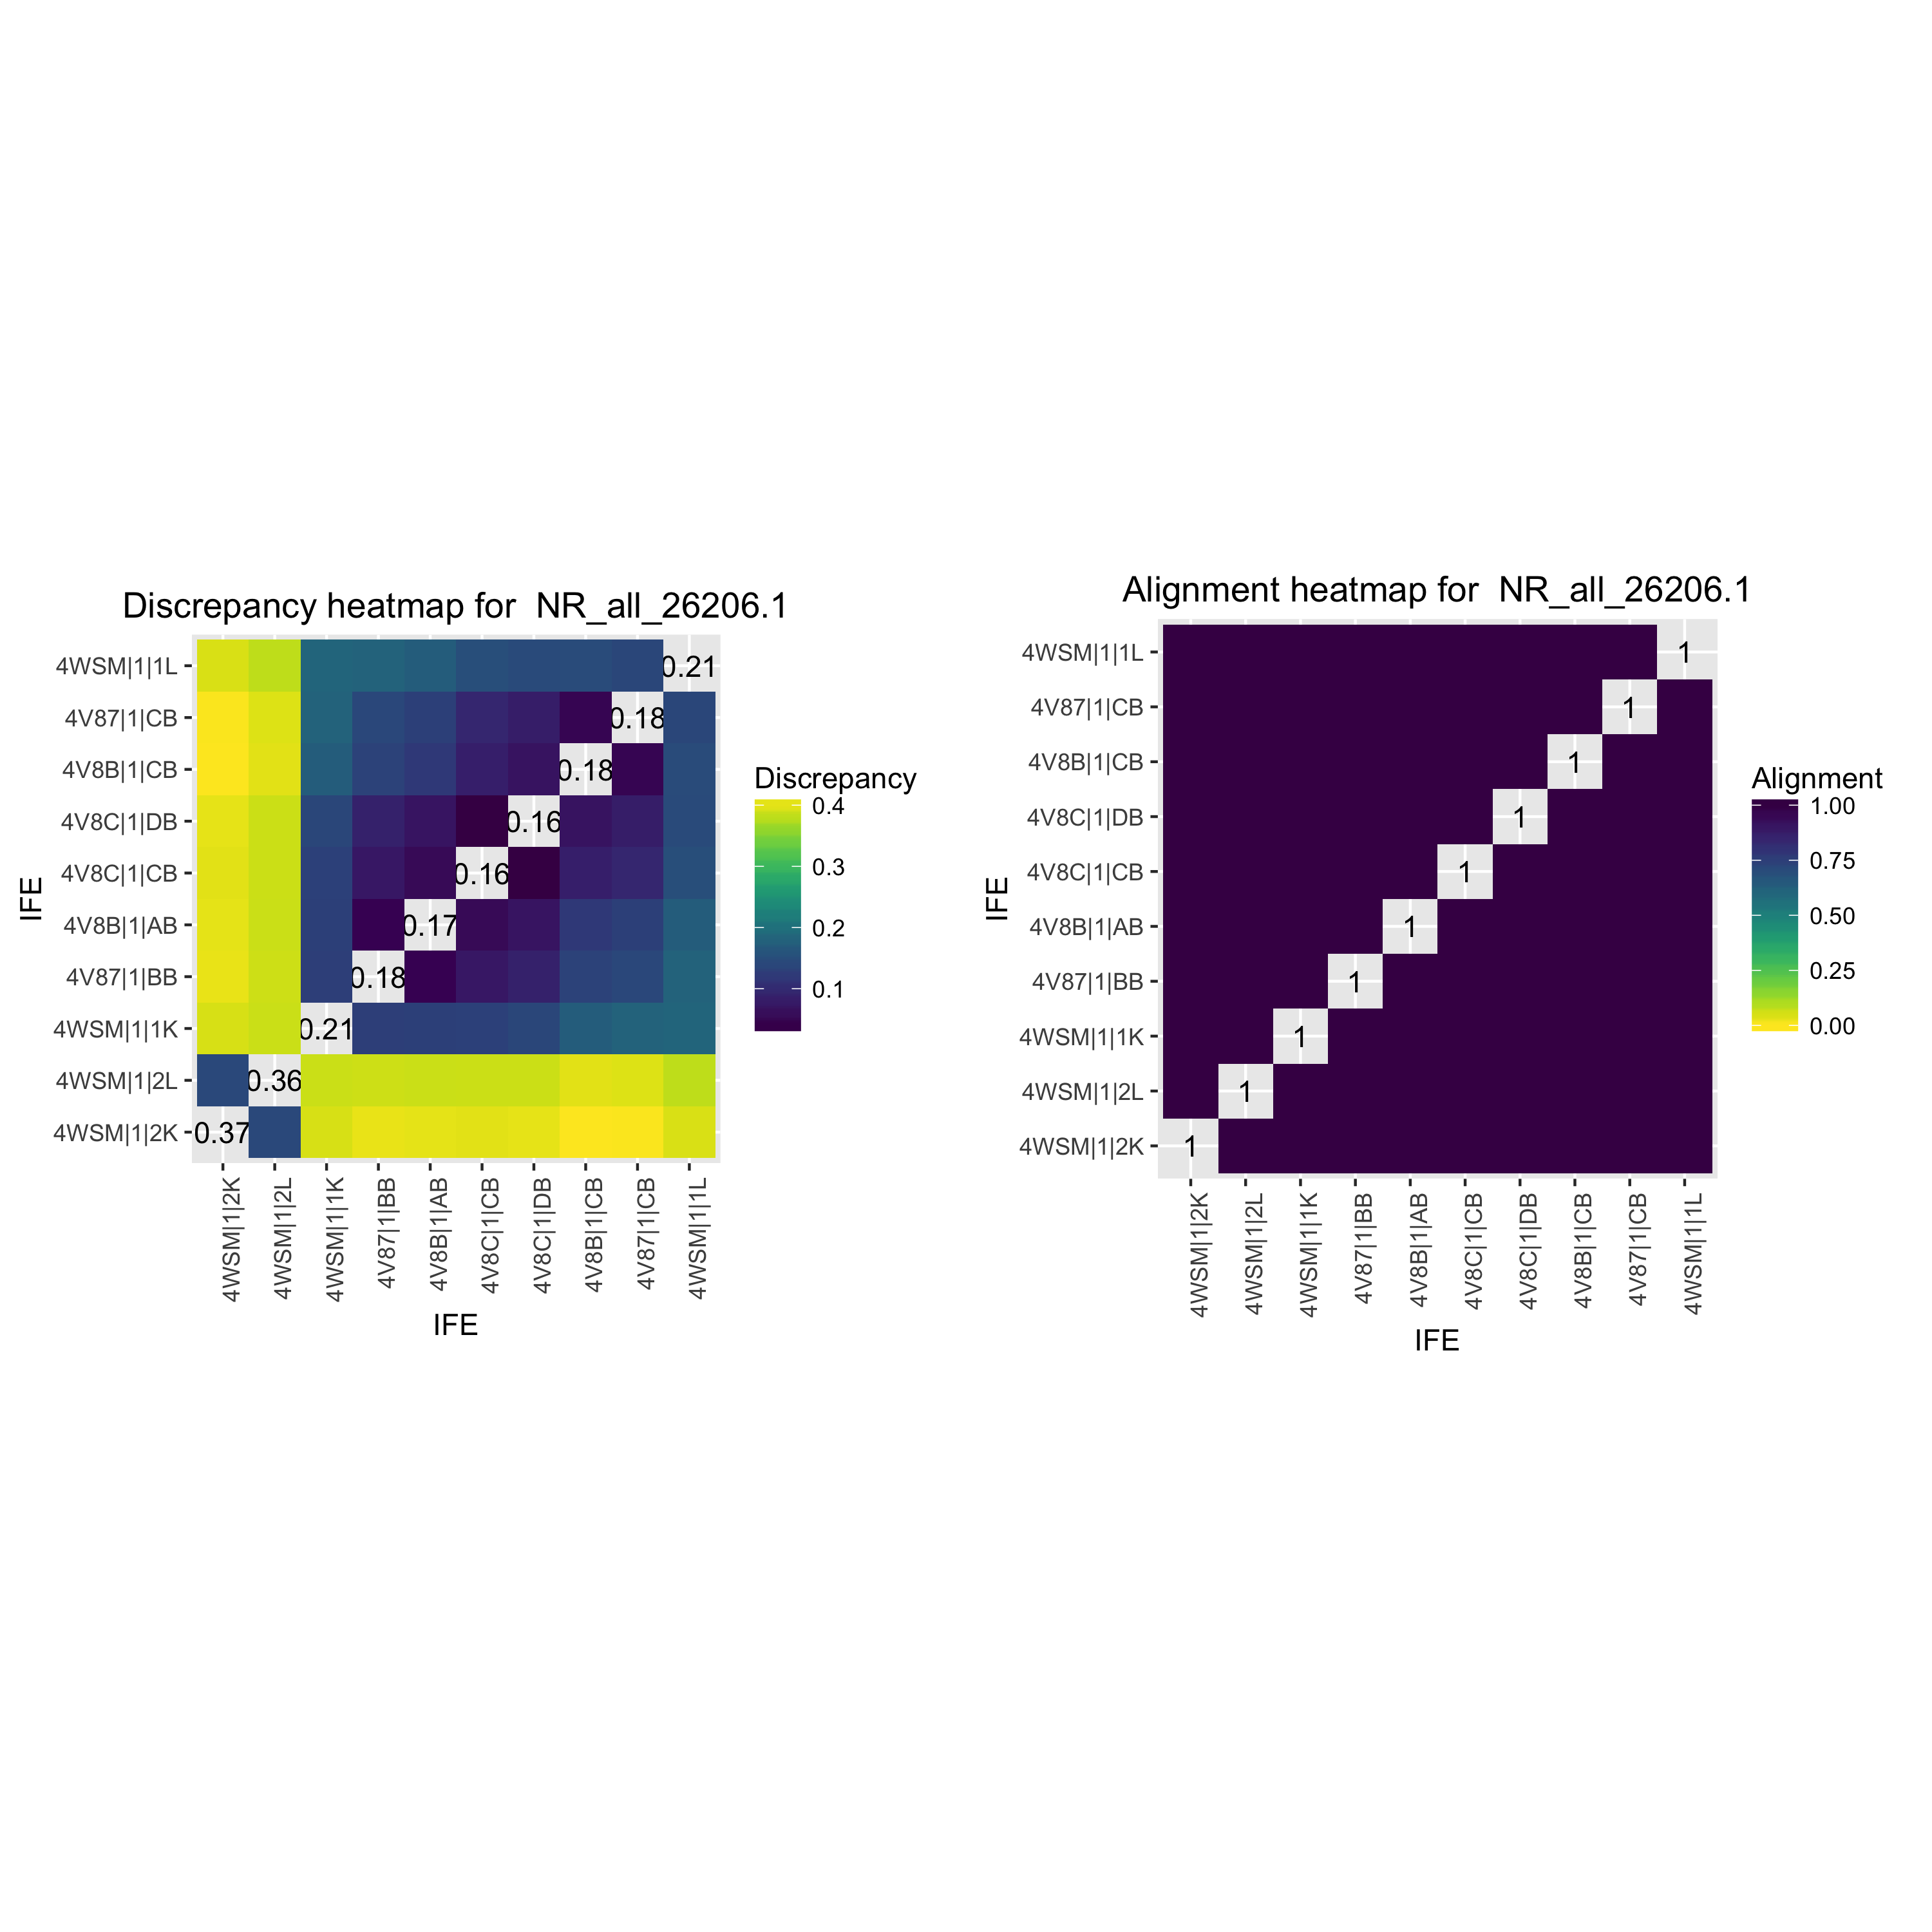
\includegraphics[width=\textwidth]{chapter-3/figs/trna-alone}
  \caption{Example of a tRNA/mRNA complex forming an equivalence class. On the
    left is a heat map of the discrepancies for all IFE’s in the group. The
    right shows the heat map of sequence similarity for the group. Color scales
    indicate the value, with lighter colors meaning ‘worse’ values. Along the
  diagonal of each plot is the mean value for each row.}
  \label{fig:trna-alone}
\end{figure}

\subsection{Protein and RNA complexes}

Small RNA/protein complexes are the groups which are most affected by usage of
discrepancy. To test how our method works we built a grouping with and without
discrepancy. We used a small, 11 nt, poly-A chain as a test case. This molecule
adopts different conformations depending upon the environment. In 4JRD it forms
a non-canonical duplex, while in 1CVJ it forms a single strand bound to a
protein. Shown in Figure~\ref{fig:small-aa-no-disc} we can see the discrepancy
of such a clustering. It contains several subgroups that are only connected
because we have not use discrepancy to split them. Upon using discrepancy this
group is partitioned into 4 other groups, one of which is shown in
Figure~\ref{fig:small-aa-disc}.  In this heatmap we can see that the group is
much more homogeneous and all pairs have discrepancy less than 0.2{\AA}/nt. In
addition all members of this group form a similar structure and are bound to
proteins, unlike the previous method where the group was a mix of single and
double stranded molecules.

\begin{figure}[h]
  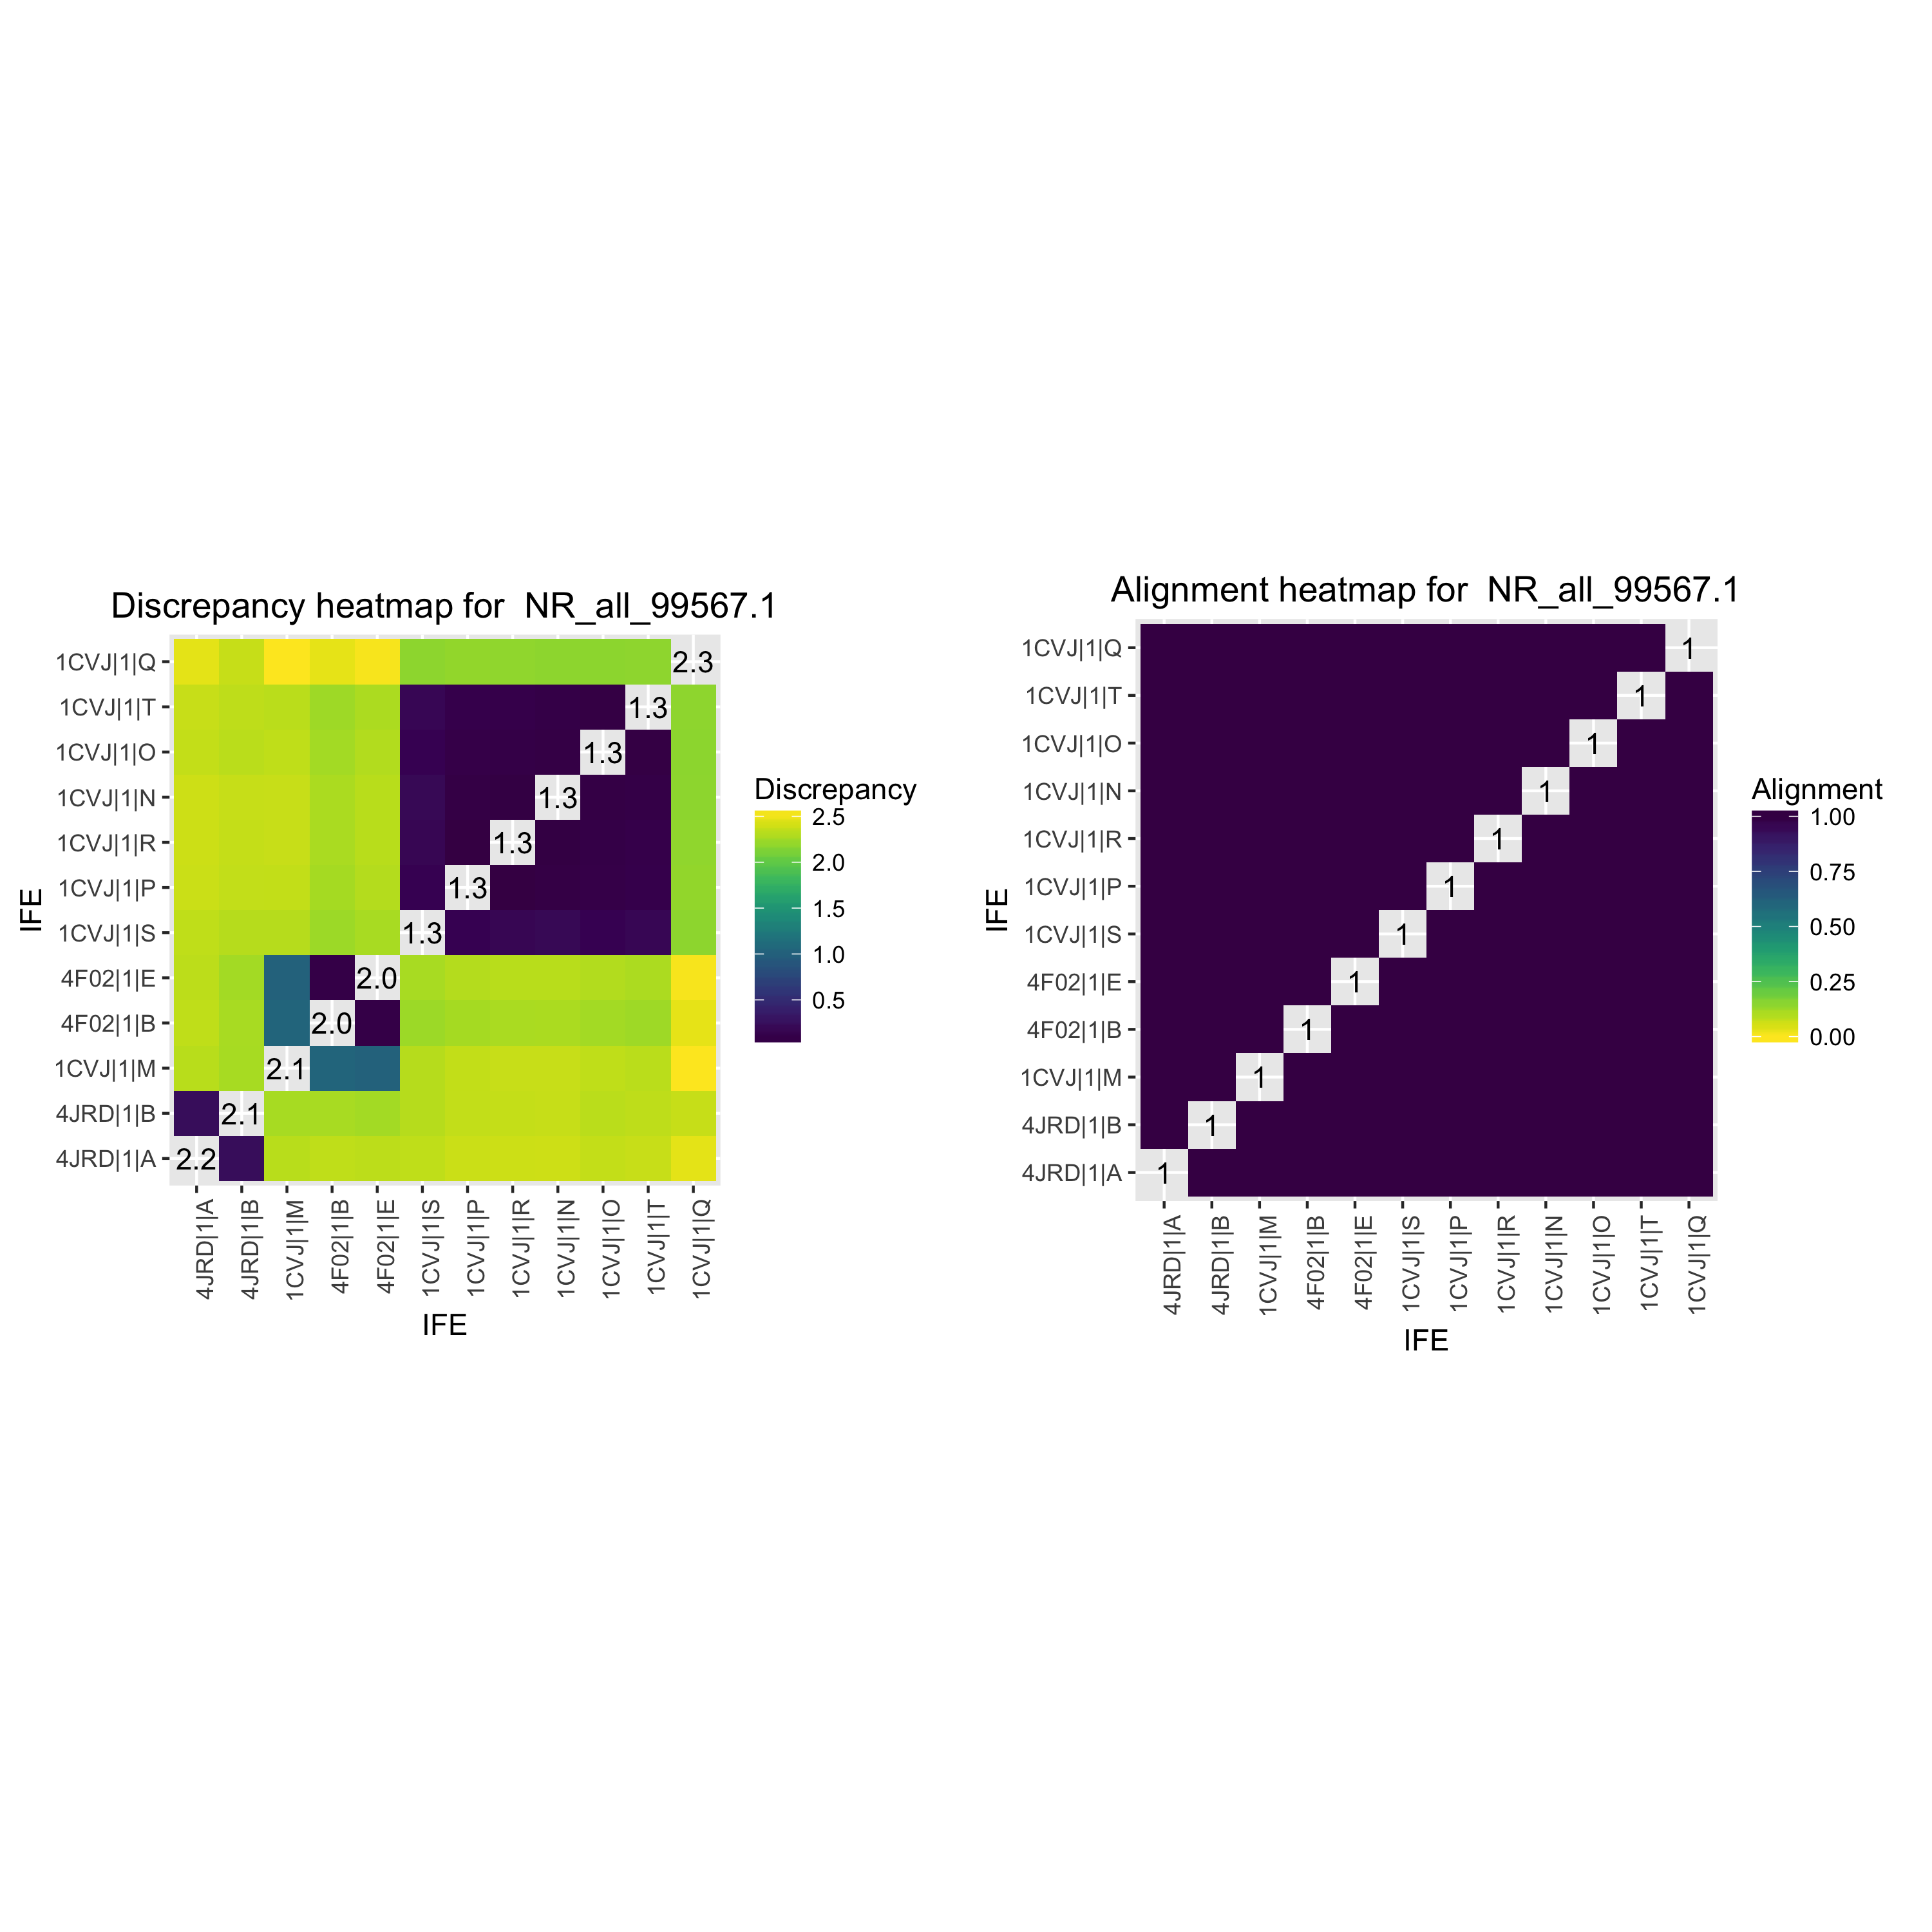
\includegraphics[width=\textwidth]{chapter-3/figs/small-aa-no-disc}
  \caption{Discrepancy heatmap for an 11-nt poly-A class built without
    discrepancy: This shows the effect of clustering a model compound without
    using discrepancy. We are showing only the discrepancy heatmap here. We can
  see that there are several subgroups with very different geometries.}
  \label{fig:small-aa-no-disc}
\end{figure}

\begin{figure}[h]
  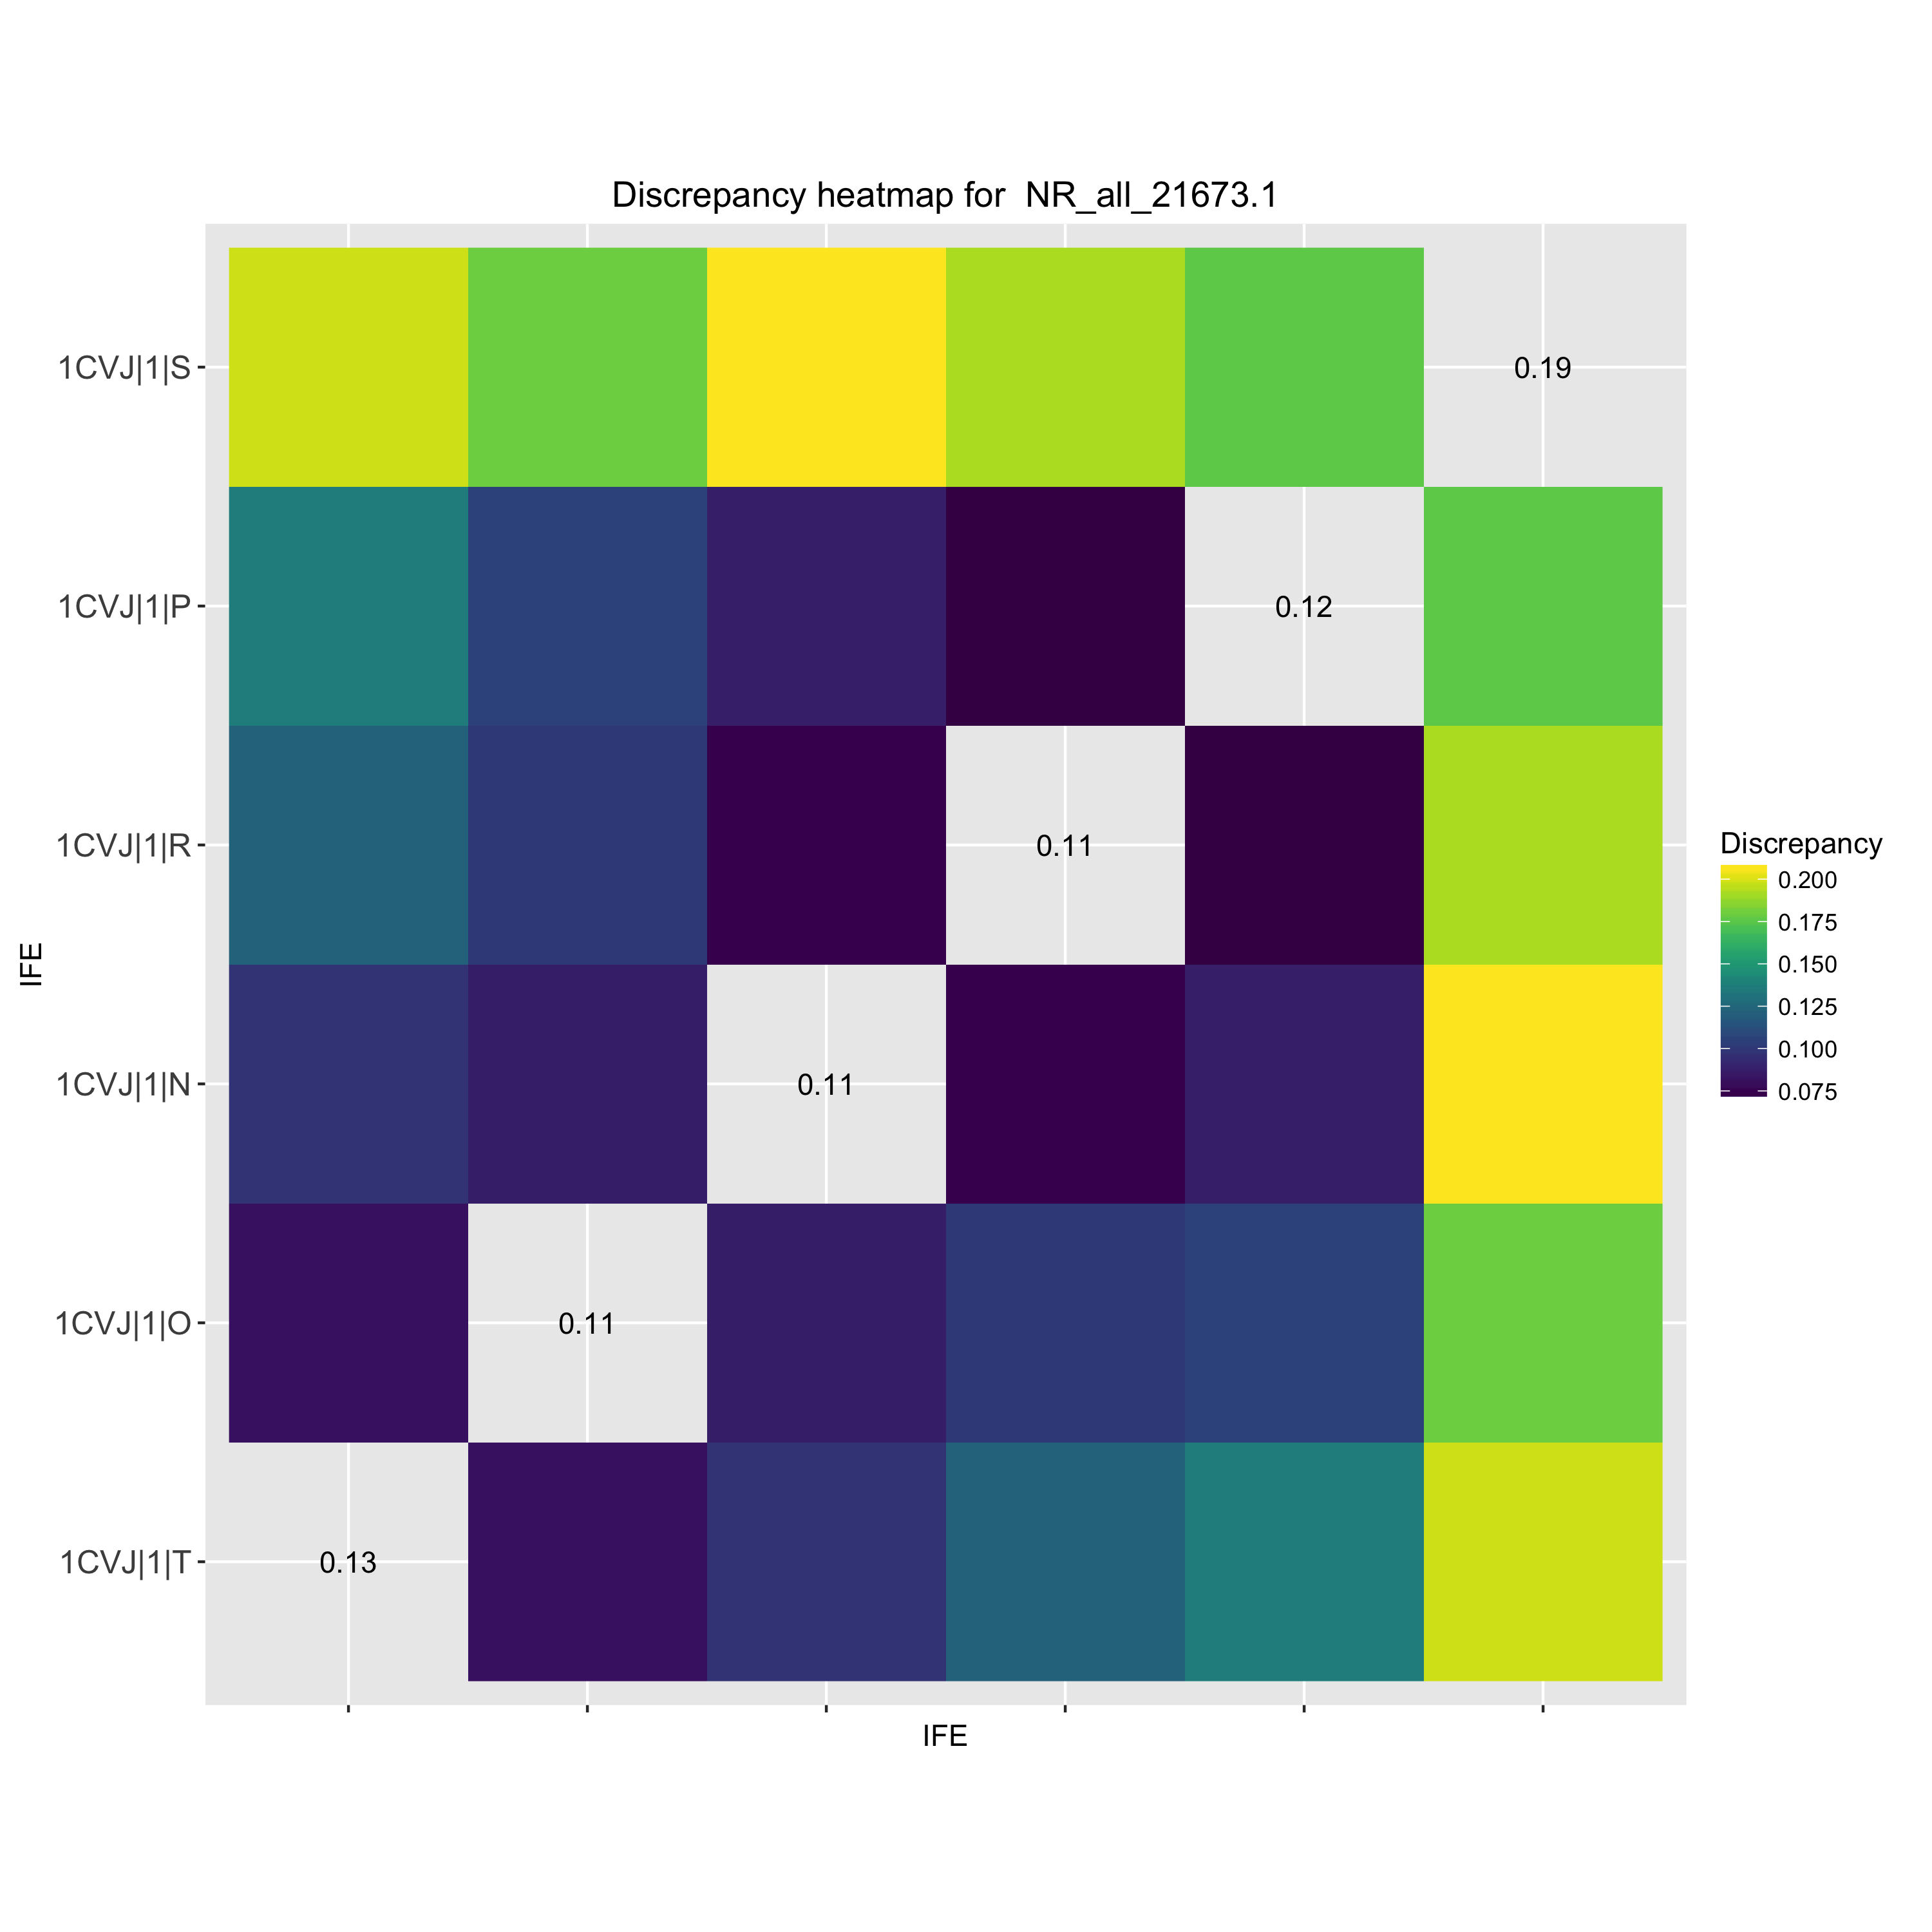
\includegraphics[width=\textwidth]{chapter-3/figs/small-aa-disc}
  \caption{Discrepancy heatmap for a small 11-nt poly-A compound built using
    discrepancy. Mean values for each row are shown on the diagonal, and the
  color scale indicates discrepancy with lighter colors being worse}
  \label{fig:small-aa-disc}
\end{figure}

\subsection{Outliers}

After evaluating specific cases we searched for outliers in our dataset. We
began by examining the distribution of maximum discrepancy and minimum sequence
similarity for all pairs in all equivalence classes. This is shown in in
Figure~\ref{fig:eq-summary}. From this figure we can see that most groups have a low
discrepancy and high sequence similarity. However, there is a very long tail of
groups with high discrepancies, some even ranging up to 4{\AA}/nt. This indicates
that some groups contain pairs of IFE's that are highly dissimilar. We call
these pairs outliers. For the purpose of this analysis we will define groups
with outliers as groups that contain pairs of IFE's with discrepancies greater
than 0.8{\AA}/nt or any group that contains a pair of IFE's that do not have a
‘good’ alignment. As discussed earlier, our criteria for chains to align well
depends on the size of the chains. For this reason we cannot use a simple
sequence similarity cutoff as with discrepancy.

\begin{figure}[h]
  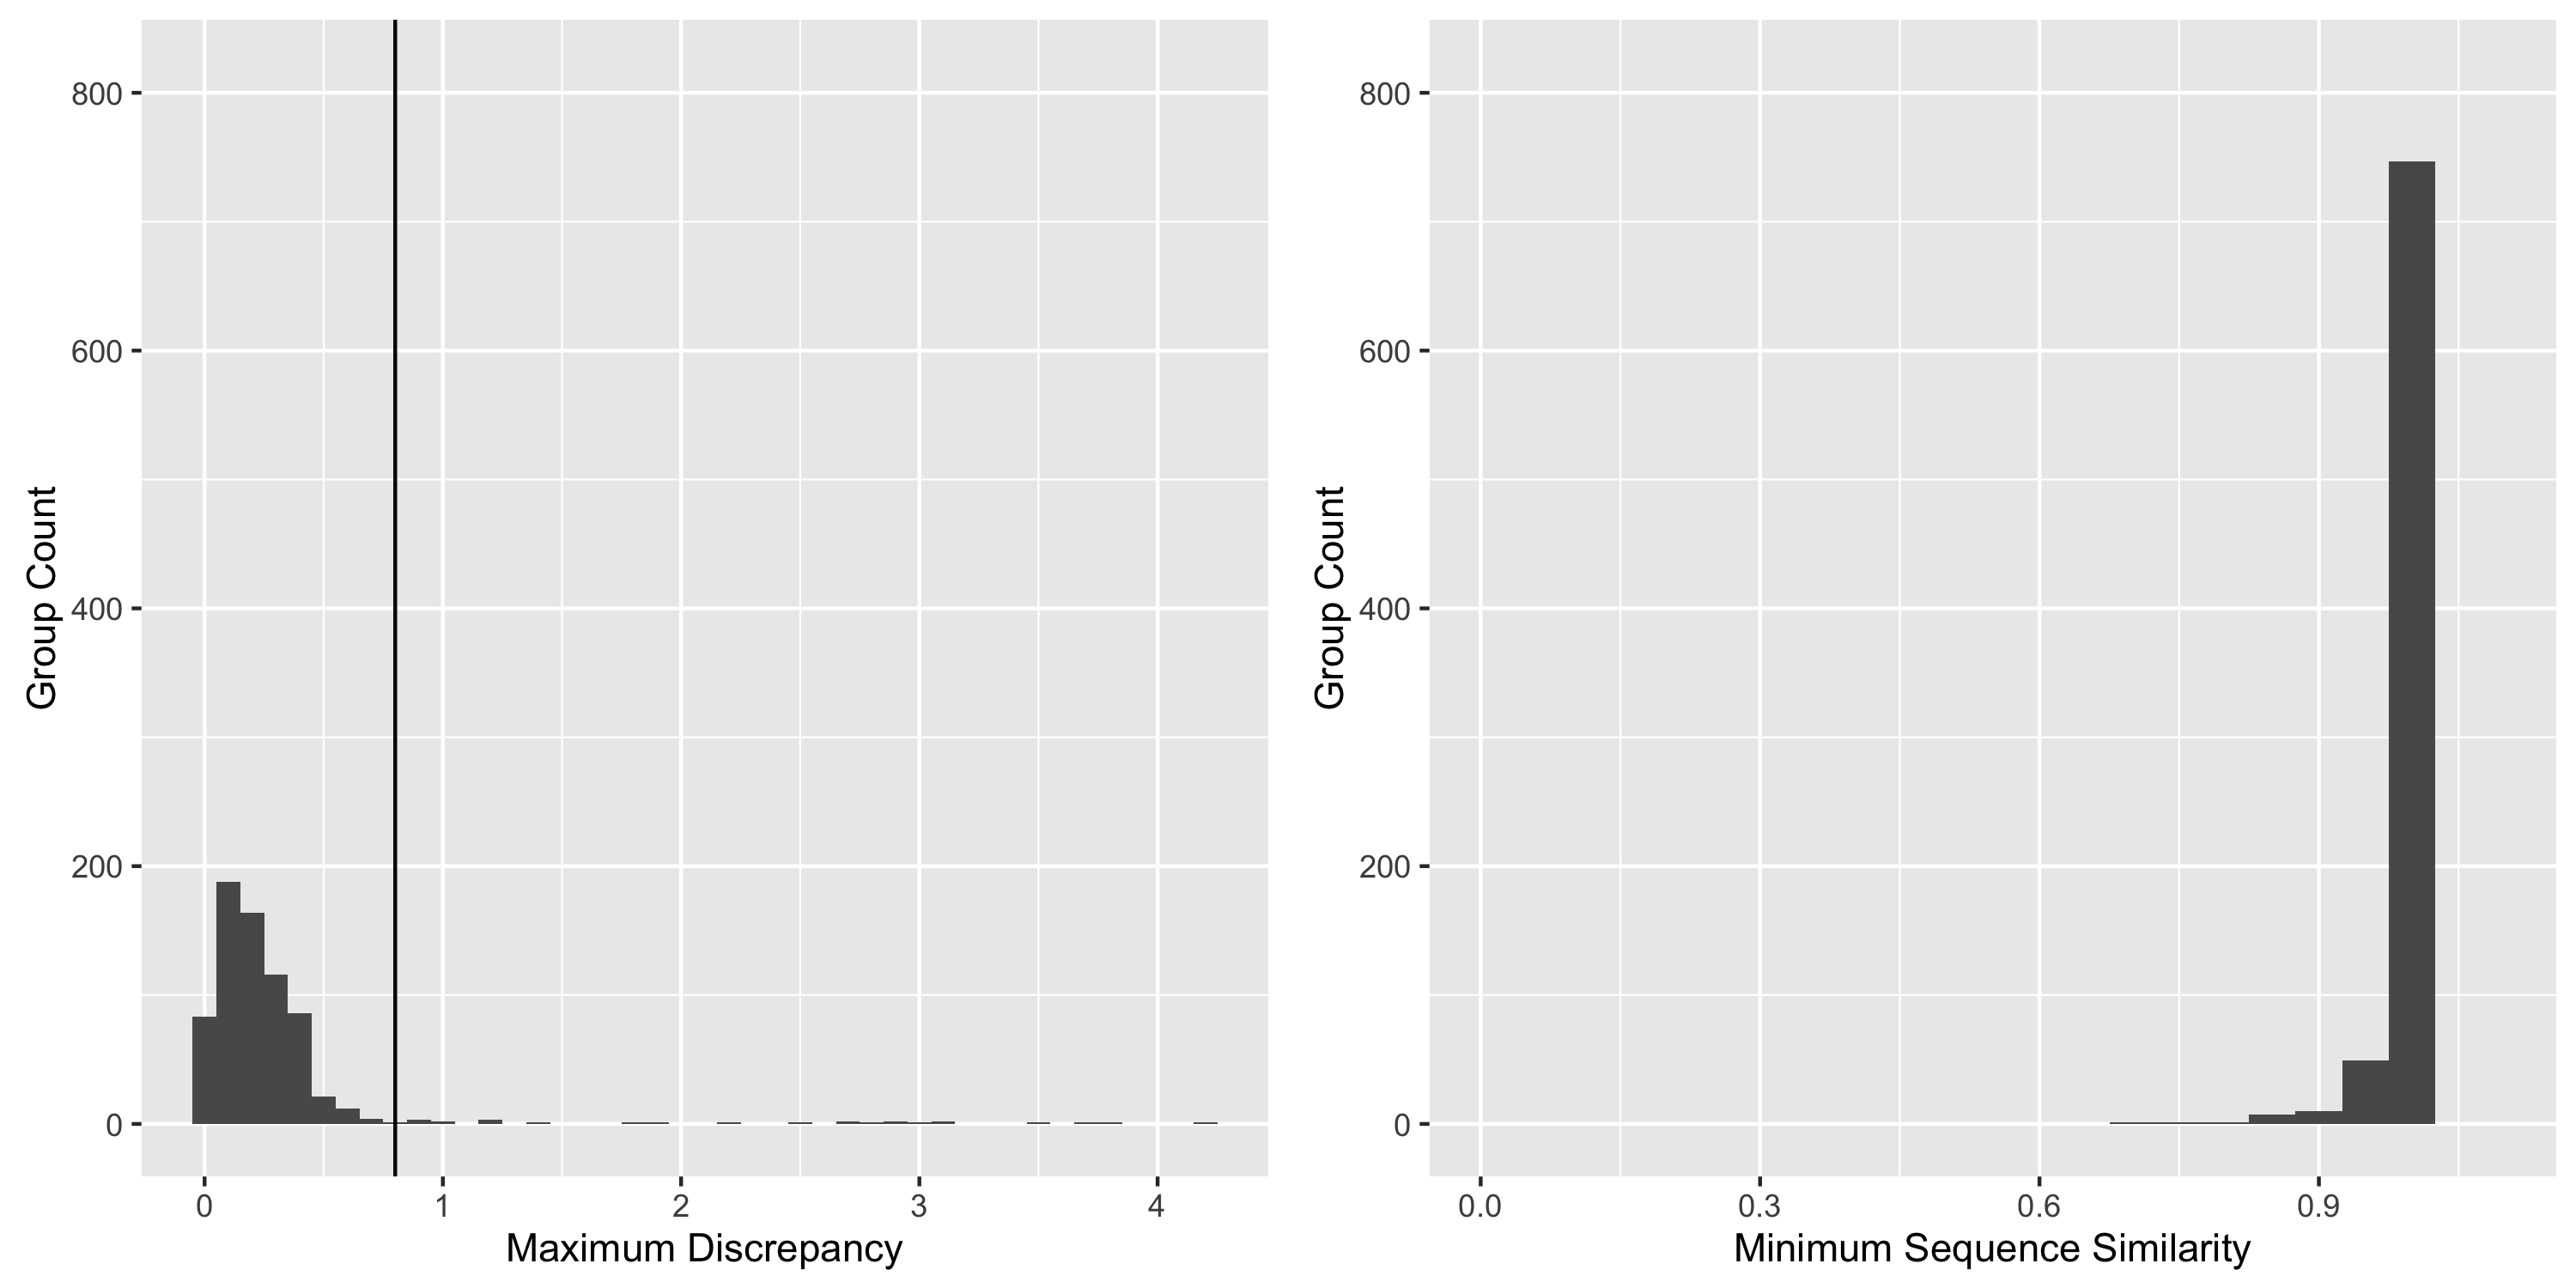
\includegraphics[width=\textwidth]{chapter-3/figs/eq-summary}
  \caption{A figure of the Maximum Pairwise Discrepancy and Minimum Sequence
    Similarity for all pairs of IFE's in all equivalence classes. The black
    lines indicate the 0.8 discrepancy cutoff (left) used a criterion for
  detecting groups with outlier pairs.}
  \label{fig:eq-summary}
\end{figure}

We then investigated the distribution of discrepancies and sequence similarities
for all groups containing outliers. The figuring summarizing this is shown in
Figure~\ref{fig:eq-outlier-summary}. This graph shows that outliers appear in all regions of
the graph. Some outliers have low discrepancy, indicating they must differ in
sequence, while others have high sequence similarity indicating they must differ
geometrically.

\begin{figure}[h]
  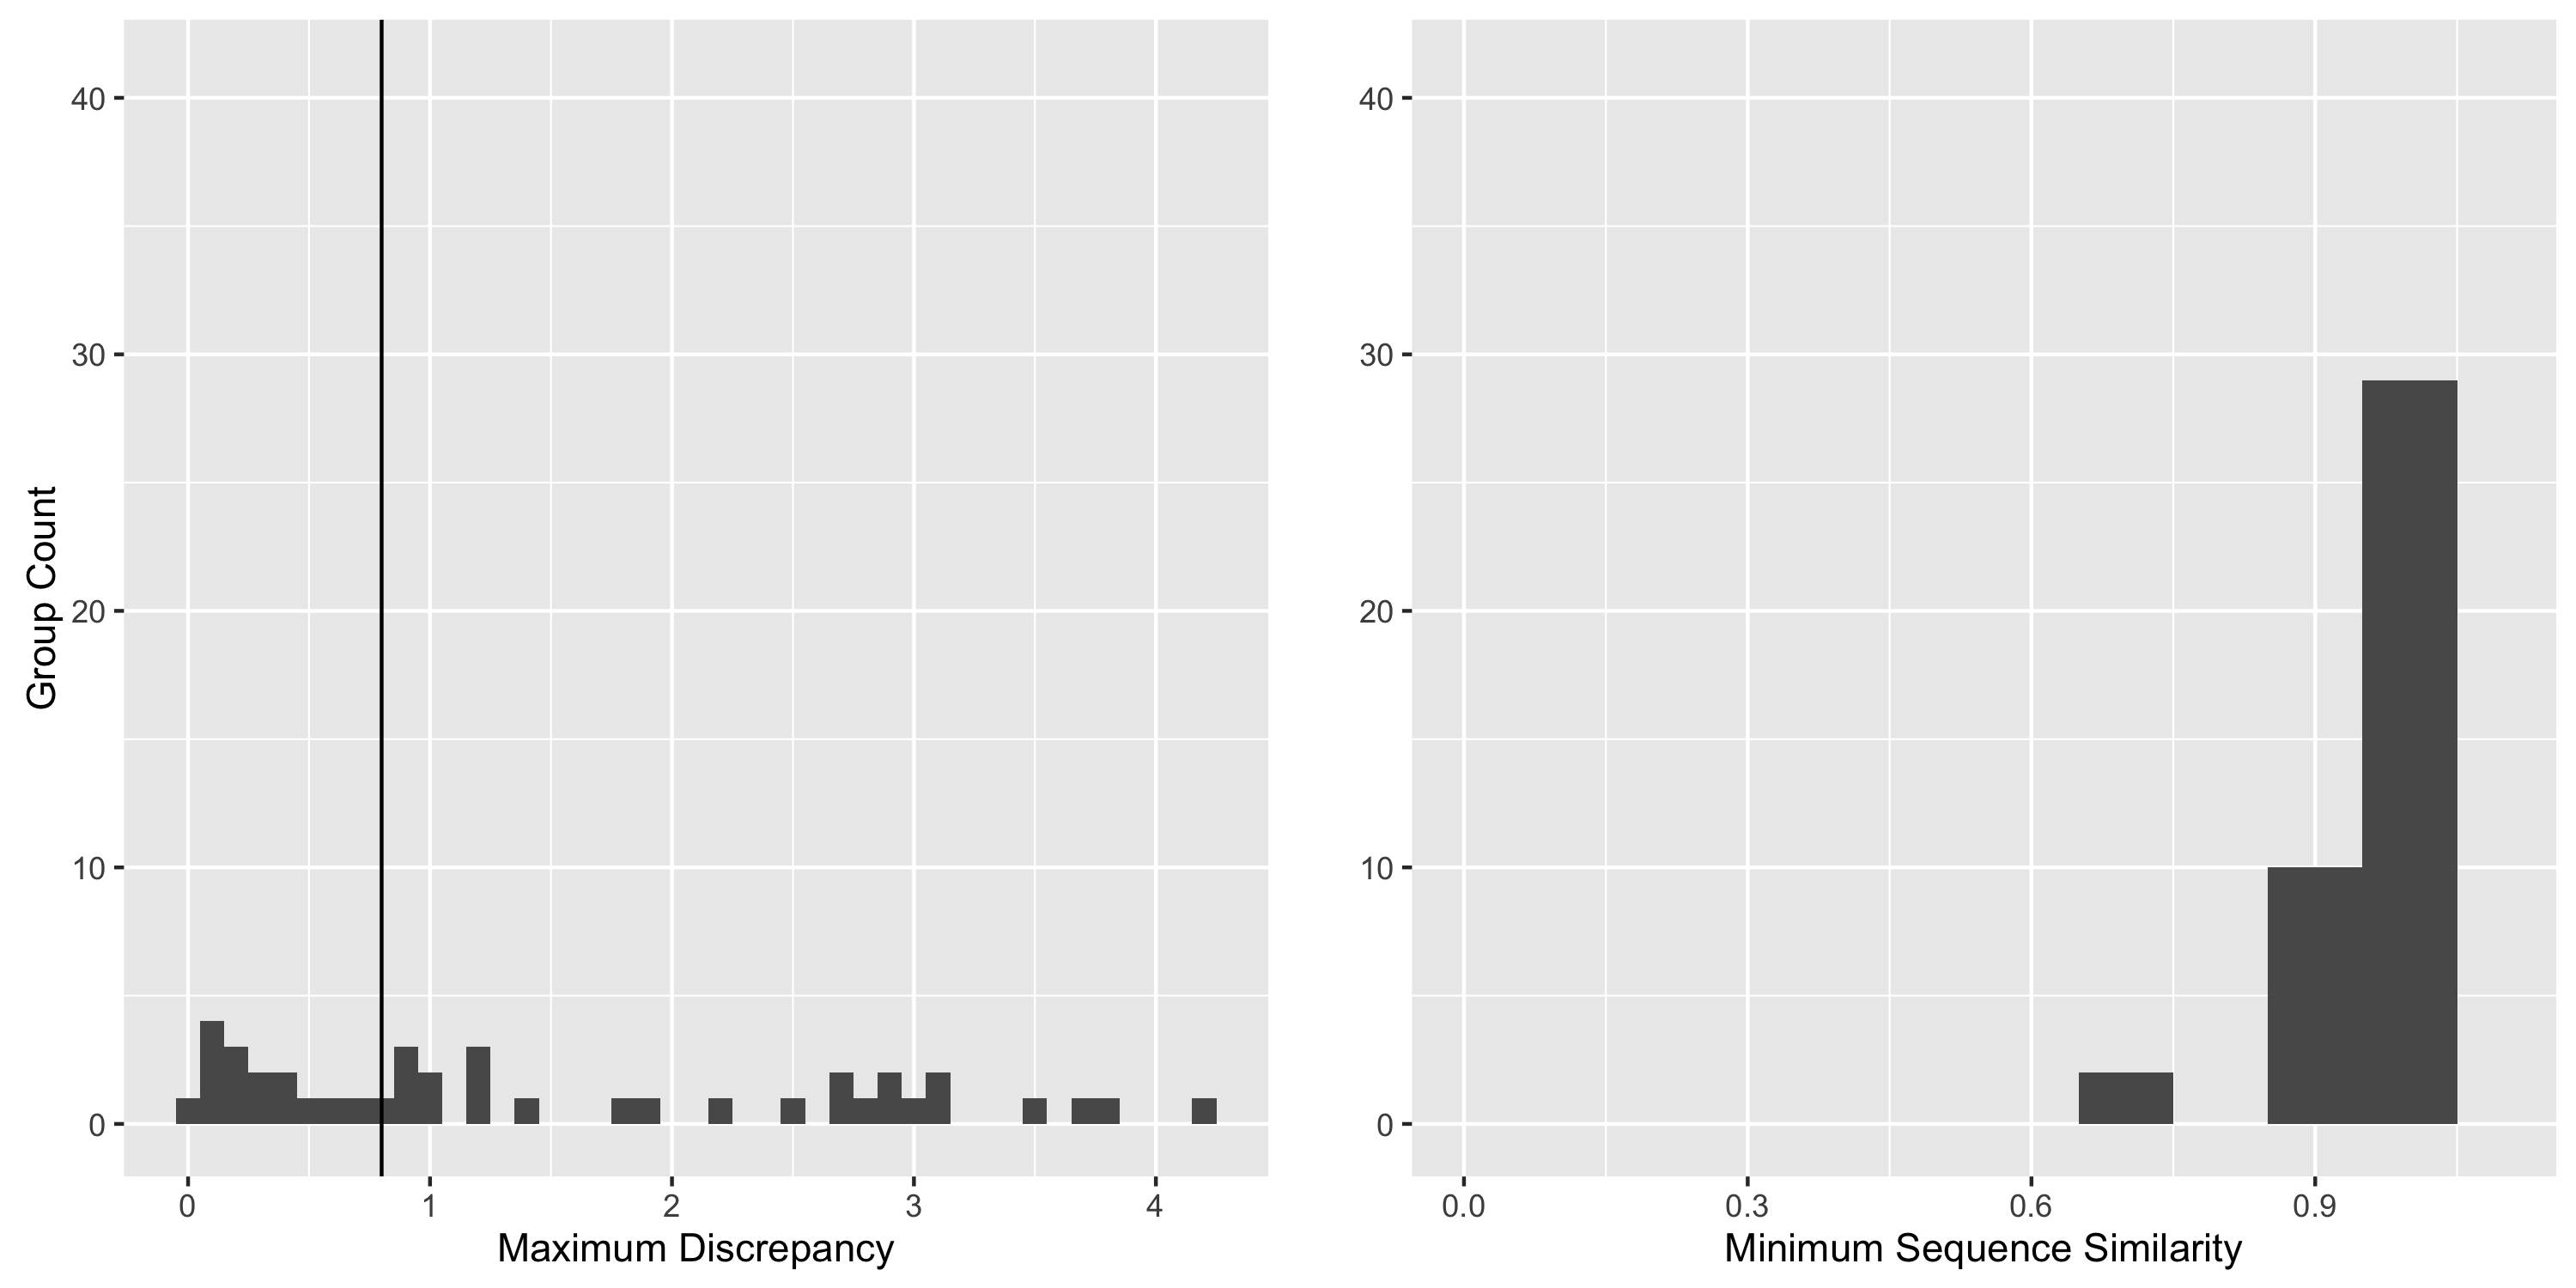
\includegraphics[width=\textwidth]{chapter-3/figs/outlier-summary}
  \caption{Discrepancy and Minimum Sequence Similarity of all groups with
  outliers. This figure shows the same data as Figure~\ref{fig:eq-summary} but
only for groups that have a pair of IFE's with discrepancy at least 0.8 or
sequence similarity less than or equal to 0.9.}
  \label{fig:eq-outlier-summary}
\end{figure}

We next examined the distribution of the number outliers, fraction of outliers,
discrepancy, and sequence similarity with respect to the size of the group in
terms of nucleotides and members as shown in Figure~\ref{fig:outlier-detail}.
This figure shows that the majority of the groups with outliers contain
relatively few members and are relatively small. However, there are a few groups
that contain many members and are large. The spike at \~80 nucleotides
corresponds to 2 tRNA groups.

\begin{figure}[h]
  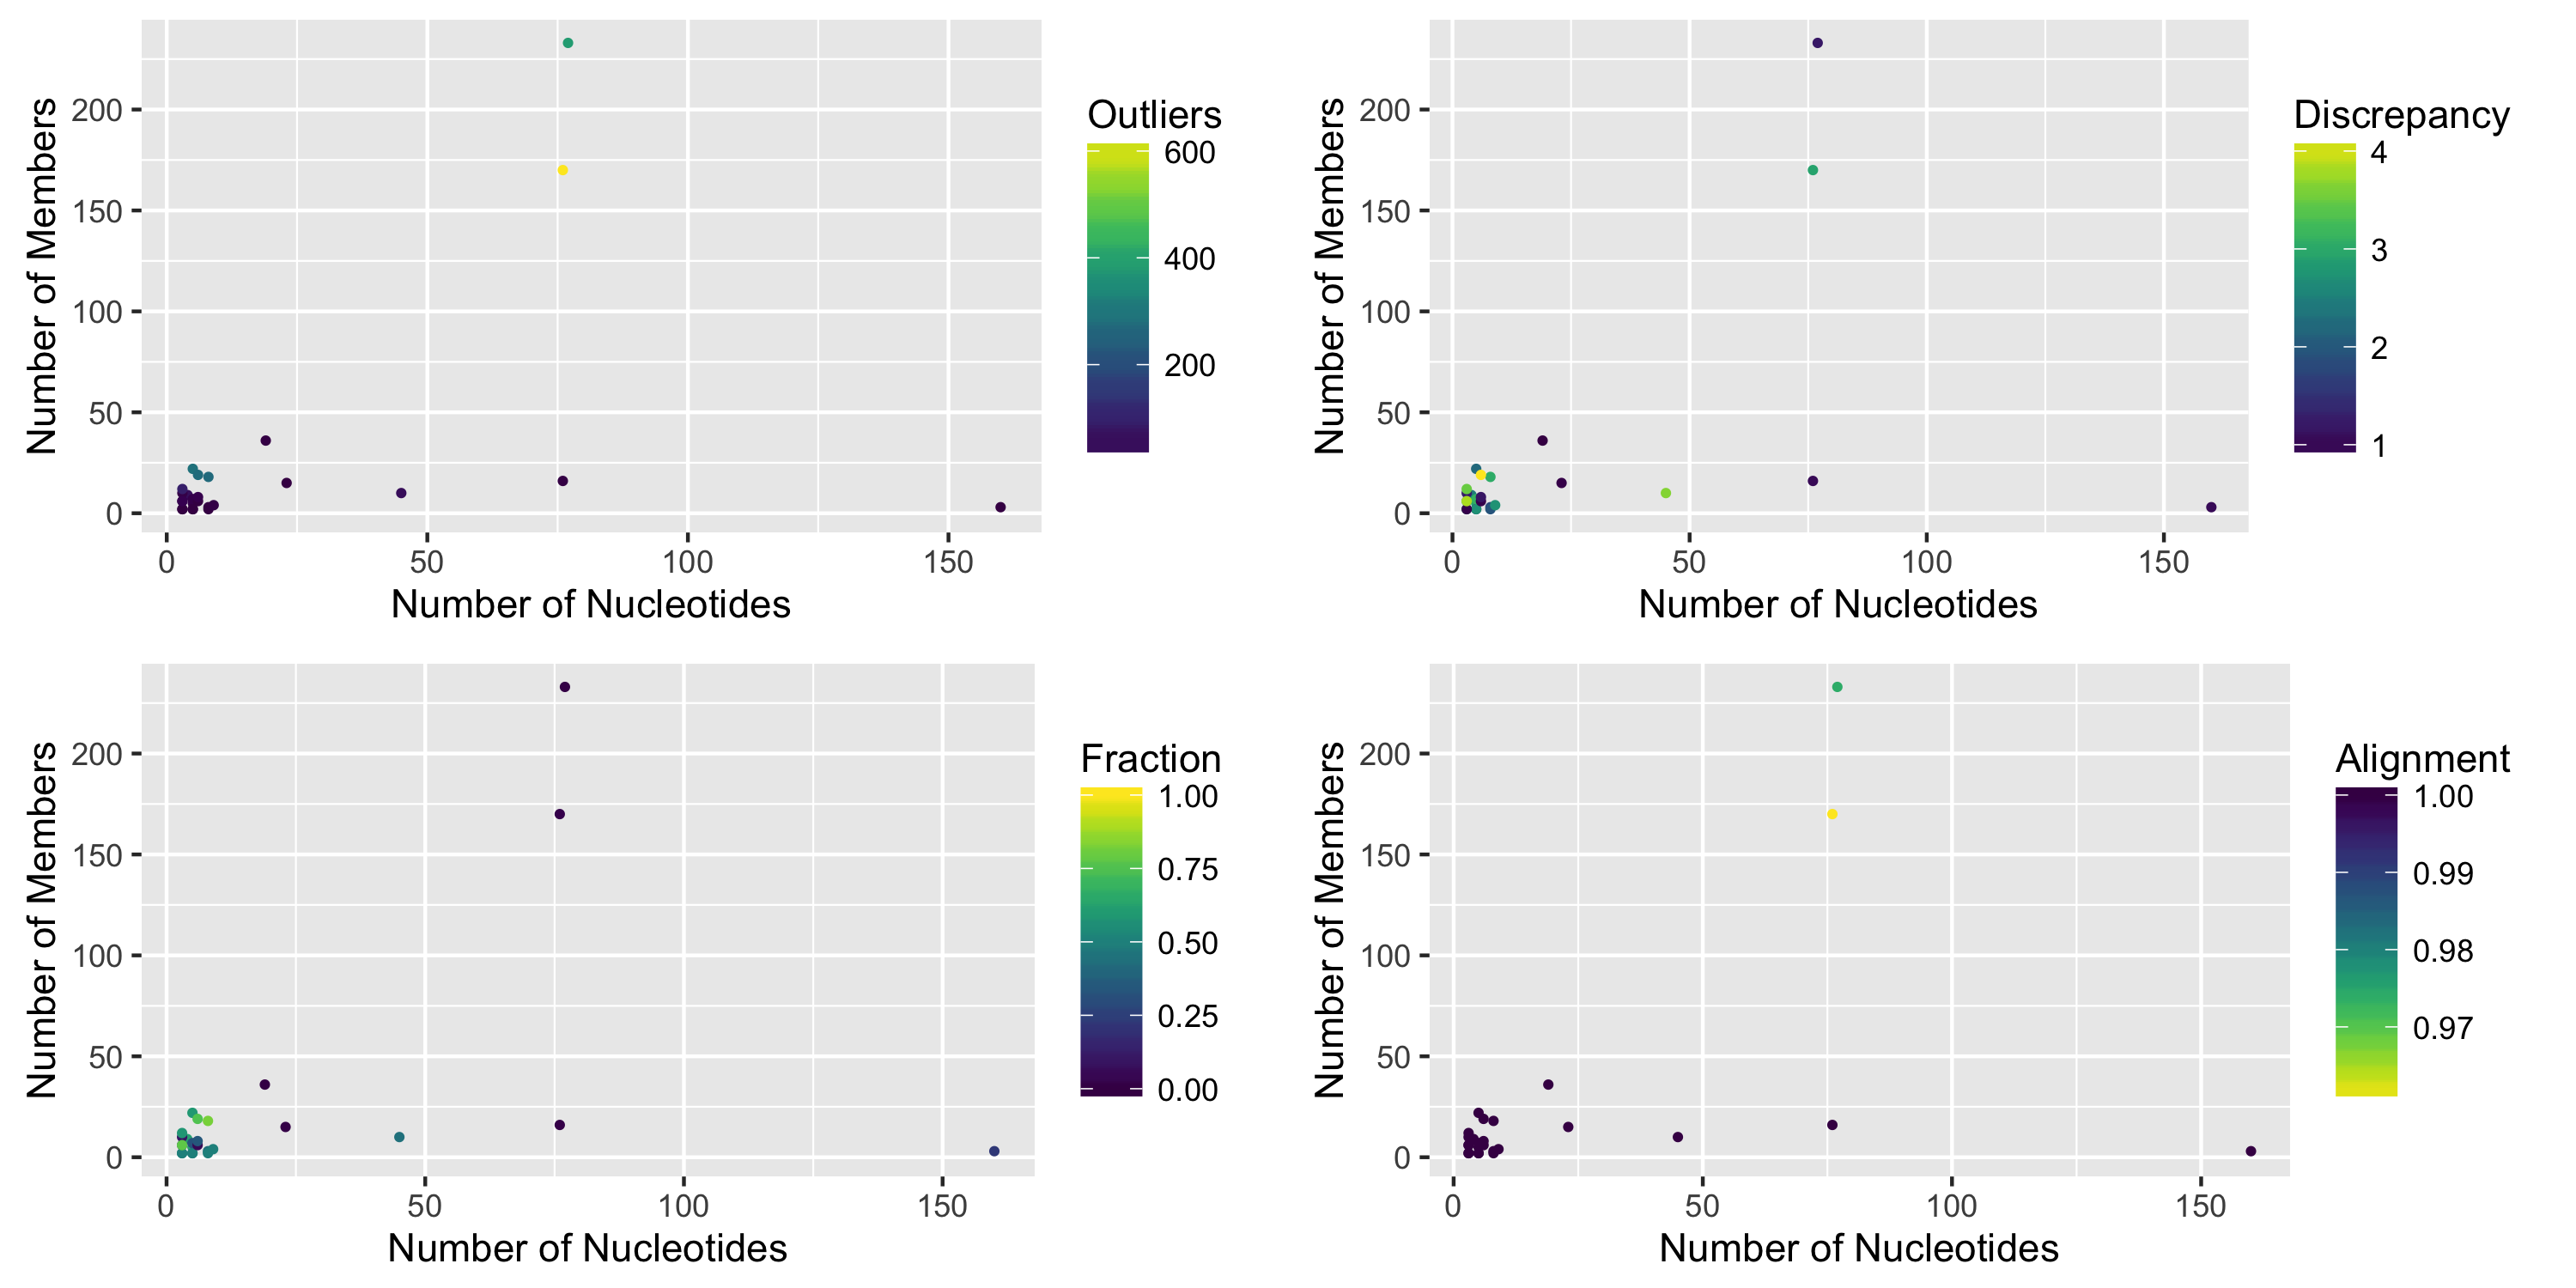
\includegraphics[width=\textwidth]{chapter-3/figs/outlier-details}
  \caption{This figure shows 4 different metrics for outliers within each group.
    Each point in all graphs represents a group that contains at least one pair
    of IFE’s that is an outlier (discrepancy greater than 0.8 or sequence
    similarity less than 0.9). In all graphs the horizontal coordinate is the
    number of nucleotides in the representative (discussed in the next chapter)
    of the group. The vertical is the number of members. The points are colored
    according to various metrics. In the upper right the points are colored
    using the number of pairs that are outliers, with lighter colors meaning
    more. Proceeding clockwise to the upper right the points are colored
    according to the the maximum discrepancy amongst all pairs in the groups.
    The lower right shows the minimum sequence similarity with lighter being a
    lower (worse) score. Finally, the lower left colors the points using the
    fraction of total pairs that are outliers, with lighter being higher
  fraction and thus worse.}
  \label{fig:outlier-detail}
\end{figure}

All groups with outliers can be classified according to the type of of outliers
they contain. The groups may contain pairs that have high discrepancy, low
sequence similarity or both high discrepancy and low sequence similarity. I
determined the counts for each of these as shown in
Table~\ref{tab:outlier-types}. This table shows that the majority of the groups,
63\%, have at least one pair with high discrepancy. The remaining 36\% of groups
contain pairs that have low sequence similarity and no pairs with high
discrepancy. I explored these classes to determine how such groups were built.

\begin{table}
  \begin{tabular}{lr}
    \toprule
    Outlier Type & Number of Groups (Percent) \\
    \midrule
    High Discrepancy & 21 (51\%) \\
    Low Sequence Similarity & 15 (36\%) \\
    High Discrepancy and Low Sequence Similarity & 5 (12\%) \\
    \bottomrule
  \end{tabular}
  \caption{This table shows the counts, and percents, of each type of outlier
  in an equivalence class.}
  \label{tab:outlier-types}
\end{table}

From the definition of our methodology, I know that all groups that contain
pairs with low sequence similarity will do so because they are connected through
a chain of high sequence similarity pairs. The NR\_all\_03381.1 group contains
protein/stem loop constructs of length 22 nt and has 4 members,
\ife{1K8W}{1}{B}, \ife{1ZL3}{1}{B}, \ife{1ZE2}{1}{D} , and 1ZE.

The other class of groups with outliers, those that contain a pair with high
discrepancy, can be caused in two ways. First, the pairs may be connected
through a chain of low discrepancies, similar to pairs with low sequence
similarity being connected through a chain of high sequence similarity pairs.
This is visible in Figure~\ref{fig:nr-all-75770.1-disc}. In this figure there are
yellow bars that only cover part of the

\begin{figure}[h]
  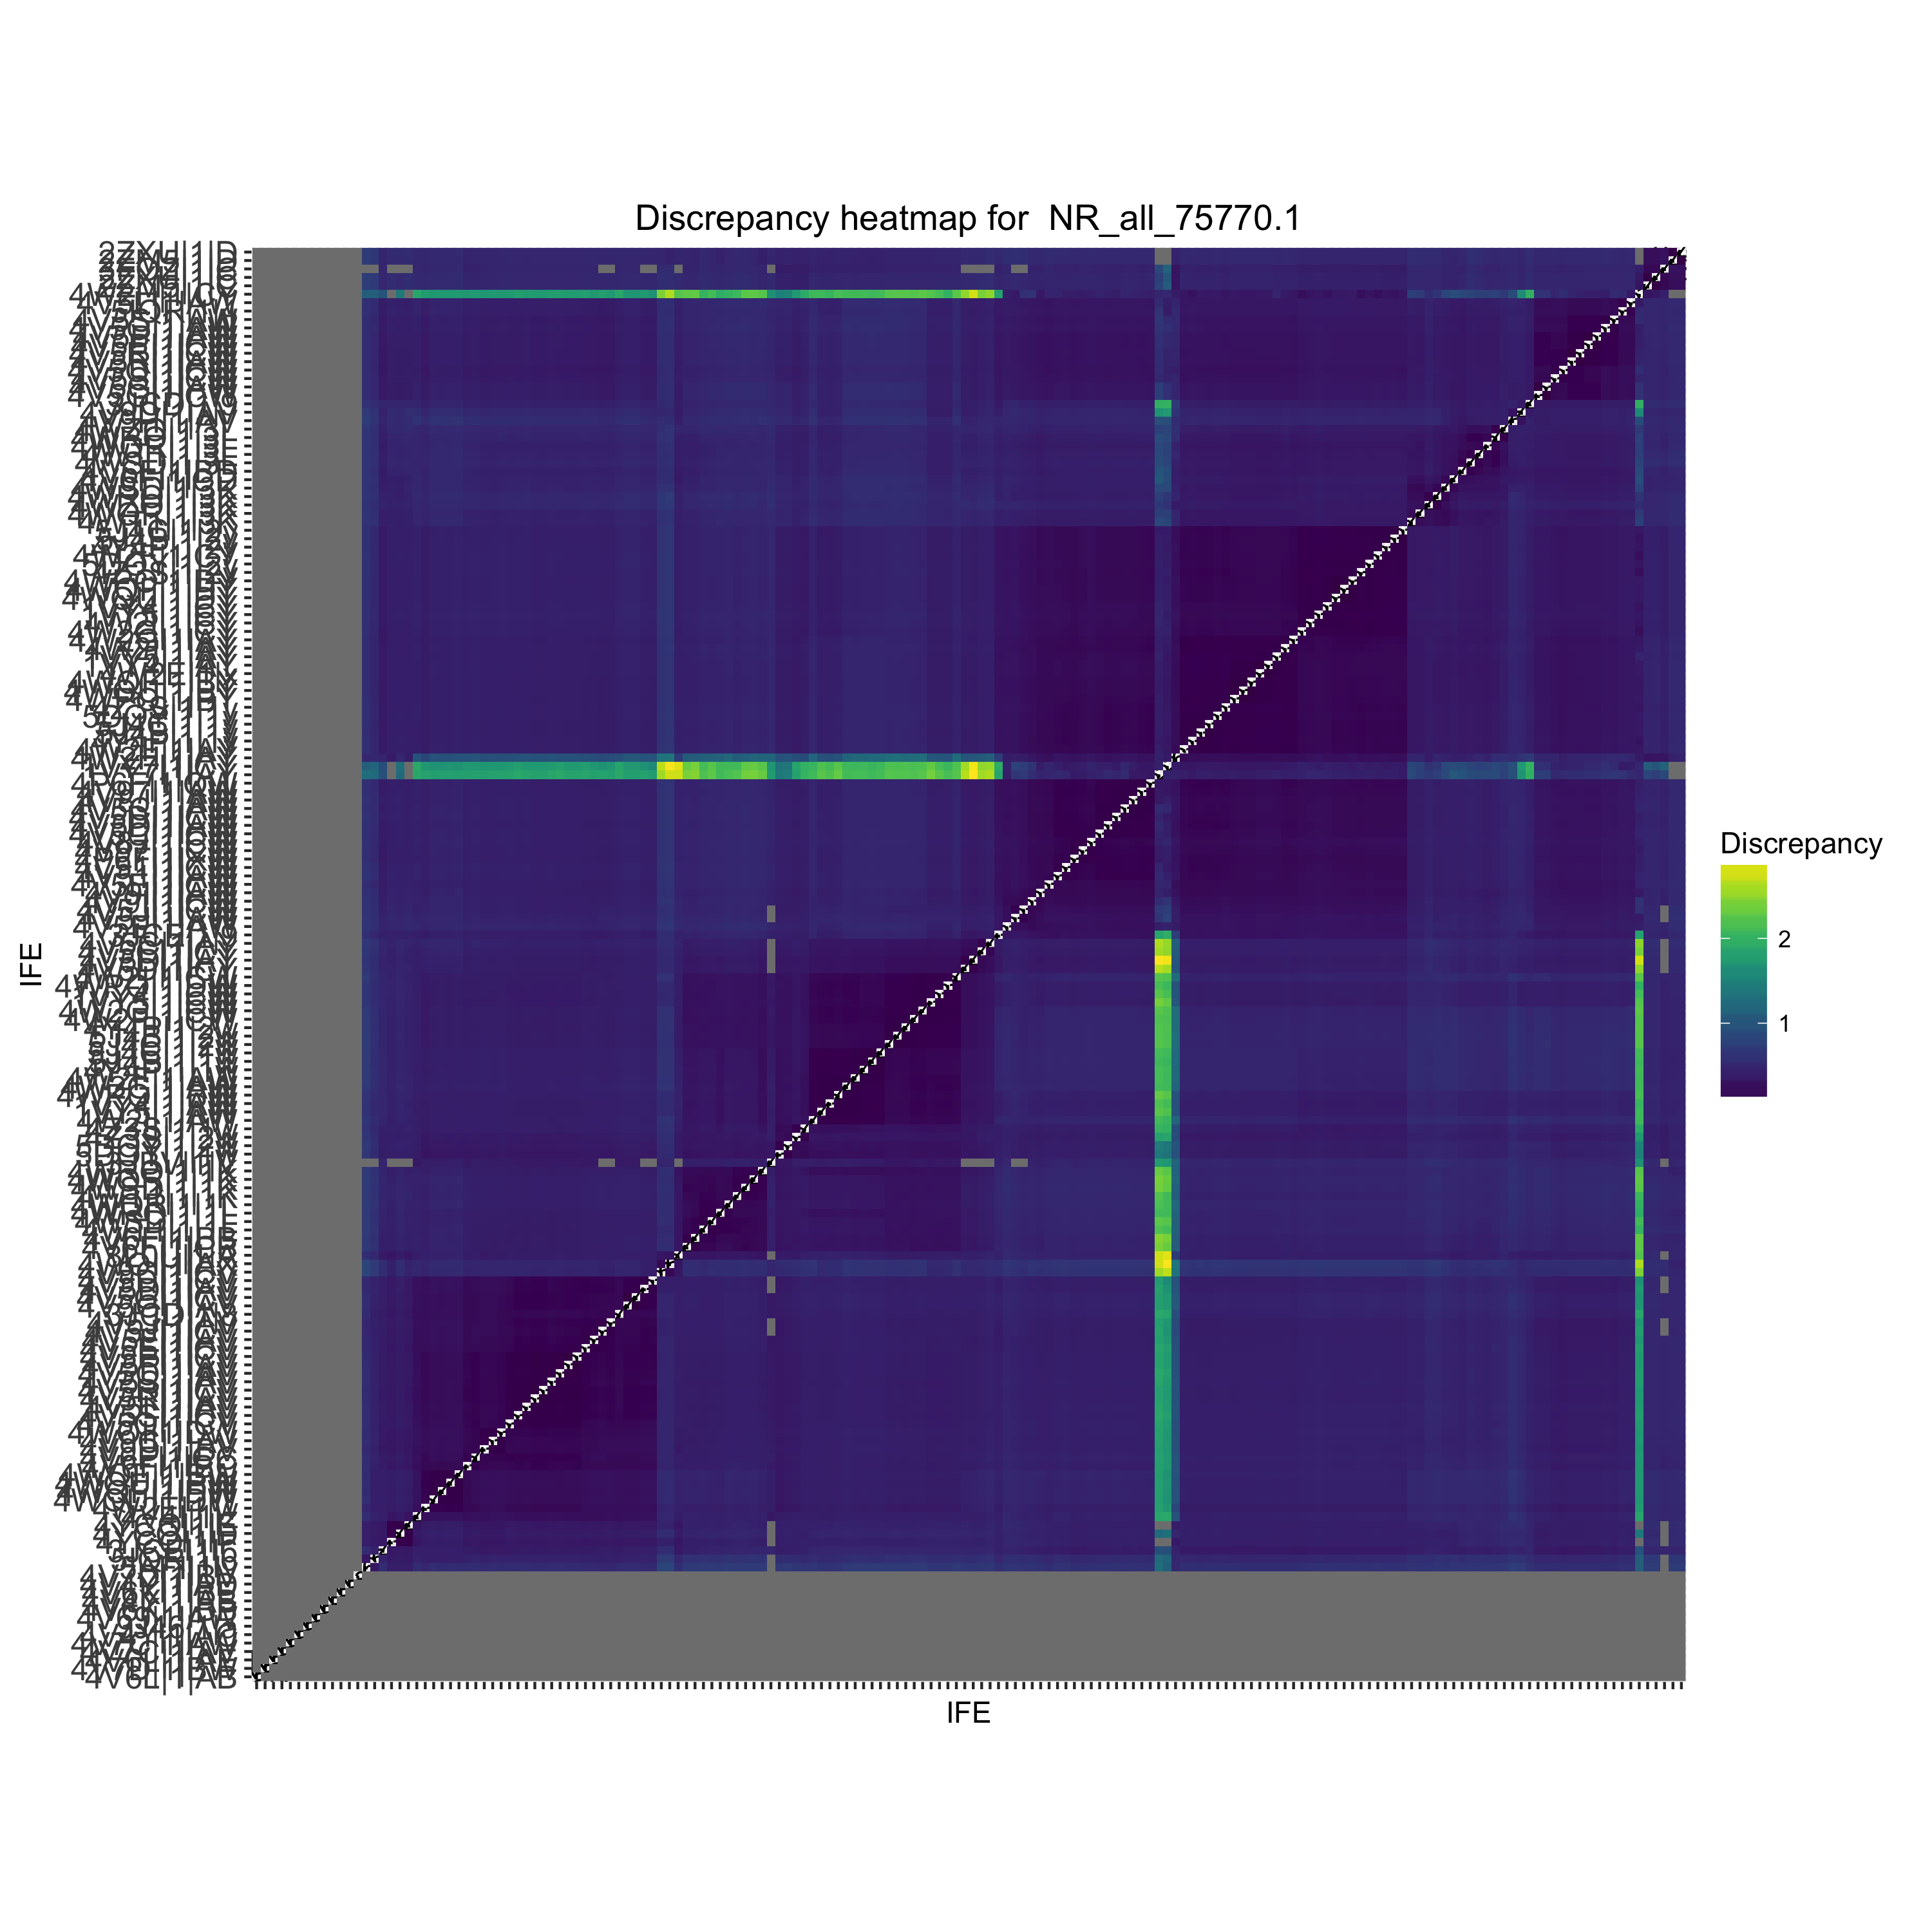
\includegraphics[width=\linewidth]{chapter-3/figs/nr-all-75770-1-disc}
  \caption{Histogram of the of the discrepancies for EC NR\_all\_75770.1, an E.
    coli tRNA group. This group contains a few IFE's which are outliers in our
  analysis.}
  \label{fig:nr-all-75770.1-disc}
\end{figure}

The other possibility is that the chains are connected through an IFE which did
not have discrepancy computed. An example of this is show in NR\_all\_18070.1
DISC. In this figure we can see a yellow line in the upper right which covers
the entire heatmap. This indicates that this IFE has high discrepancy to all
other members of the group. This IFE is connected to all other members through
the IFE’s that have no discrepancy shown (grey bars).

We examined the two groups, NR\_all\_18070.1 and NR\_all\_75770.1 manually and found
that they are tRNA groups. We will look at NR\_all\_18070.1 first, which is a tRNA
group with 233 members and is the highest point on the summary graphs. Shown in
Figure~\ref{fig:nr-all-18070.1-disc}. The outliers are due to a single IFE which is a
truncated tRNA. While it is somewhat structurally different from all other
members it is very similar in sequence. Because these molecules are uncommon and
it is still similar enough to rest of the group to ‘belong’. It is connected to
the rest of the chains through IFE’s which have no computed discrepancy.

\begin{figure}[h]
        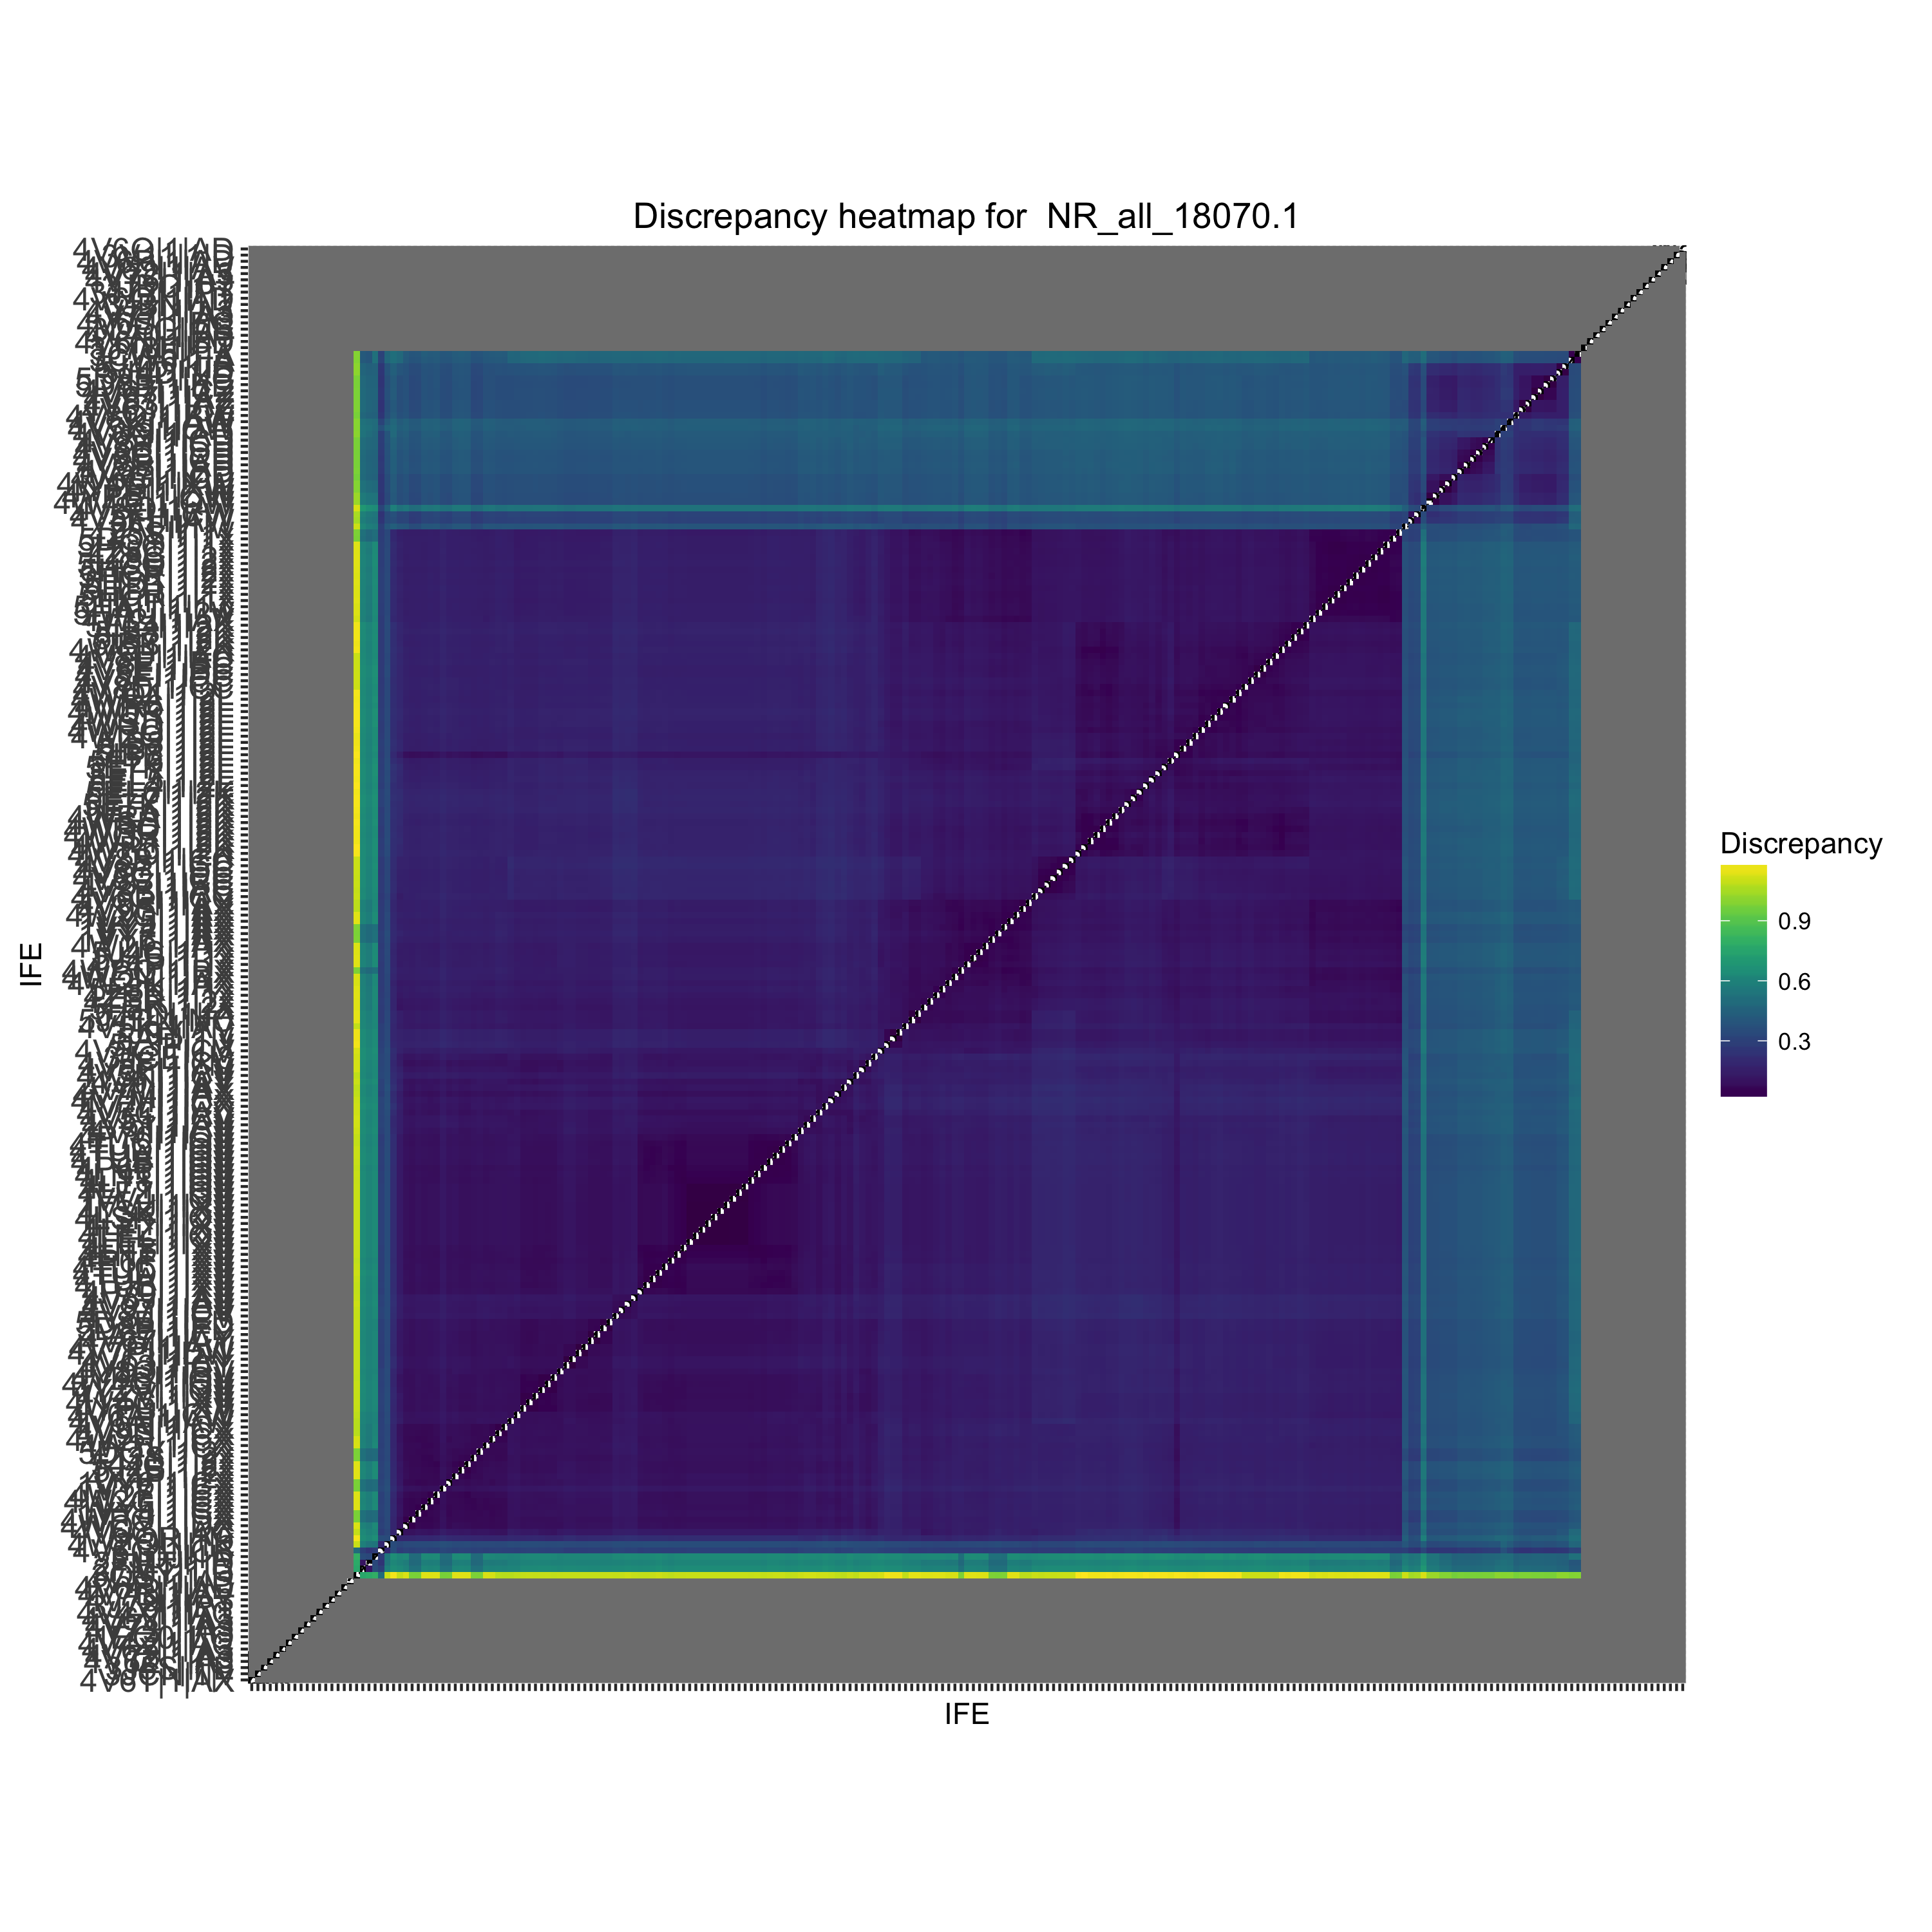
\includegraphics[width=\textwidth]{chapter-3/figs/nr-all-18070-1-disc}
  \caption{Figure summarizing the discrepancy heatmap for all IFE’s in
  NR\_all\_18070.1, a tRNA group with 233 members. }
  \label{fig:nr-all-18070.1-disc}
\end{figure}

The second NR\_all\_75770.1 is the second highest point on these plots. It is an
E. coli tRNA group with 170 members. There are a few IFE’s which are outliers
relative to the rest of the group. These chains appear to be fragments of the
larger tRNA. For example 1VY7 is a 5 nt fragment of the 76 nt tRNA.

We manually investigated the other groups with outliers and found that the
outliers are often placed into the same group because there is a structure that
we do not compute discrepancy for, such as a low resolution X-ray, that connects
the outliers to the rest of the group. For example, in previous version where we
did not compute discrepancy for NMR structures, an HIV hairpin would get joined
with a duplex of the same sequence because there was a NMR structure. All three
types of chains, the duplex, hairpin and NMR structure contained the same
sequence and thus were joined on the basis of sequence similarity. This was
resolved for NMR structures with the usage of discrepancy for them as well.
However, it remains an issue for low resolution X-ray and crystallography
experiments.

\section{Conclusions and future extensions}

Overall our grouping methodology successfully groups all chains into equivalence
classes. Our methodology is an improvement over the previous approach for
several reasons. First, it can work with mmCIF data by not only cluster the
largest chain in a file. Secondly, it computes and all discrepancies and
alignments to allow for future tuning of the parameters. Finally, our method
does not compute discrepancies for low resolution structures which will show
artificially high values.

There are several improvements that should be made. Notably, our method of
geometric similarity, discrepancy, is flawed for this task. It is too sensitive
to poor modeling in structures. Often the issue is the bases in nucleotides have
unusual orientations. If this was replaced with a different method that is less
sensitive to base orientation it may be possible  to compute all geometric
comparisons.

In addition, while evaluating the methodology it has been very useful to compute
a grouping using only sequences and then examine the changes when discrepancy is
applied. This could become part of the standard clustering procedure. For
example it may be useful to create a series of groupings built off each other.
The first a simple sequence only building, then adding species constraints, then
finally adding the discrepancy comparisons. This would make it easier to examine
our methodology as well as provide information about the linkages, if any
between groups. For example, there are likely many small groups that differ
structurally but have the same, or very similar sequences. Such groups may be
interesting for researchers interested the range of structures a single sequence
can form. A hierarchy of groupings could make this easier to determine.

Finally, small structures may well require a different set of rules for
comparison grouping. The work here was guided strongly by our experience with
ribosomes and tRNA molecules. These are much larger and show much clearer
differences than small synthetic molecules. It may be worthwhile to focus
exclusively on the small molecules to improve the methodology. For example, we
currently only use one chain when making geometric comparisons. This works well
with large molecules buy may not be accurate for small synthetic compounds. In
addition, it may be better to allow small chains to join through non-canonical
pairs as well as canonical cWW pairs. Doing so could allow us to build better
groups for the poly-A duplex or G-quadruplexes more accurately.
